% =====================================================================
% Judging the Step, Not the Answer — v3 full draft (structure v3.1a)
% Placeholders: \PH{ID} — enumerated in PLACEHOLDERS.md. Numbers from
% the registry are final; placeholder-marked items are listed separately.
% =====================================================================
\documentclass{article}
\IfFileExists{iclr2027_conference.sty}{\usepackage{iclr2027_conference}}{%
  \usepackage[margin=1in]{geometry}\usepackage{natbib}\newcommand{\iclrfinalcopy}{}}
\usepackage{times}\usepackage{amsmath,amssymb}\usepackage{booktabs}
\usepackage{graphicx}\usepackage{url}\usepackage{xcolor}\usepackage{colortbl}
\graphicspath{{assets/}}
\usepackage[hidelinks]{hyperref}
\newcommand{\ptrue}{P(\text{True})}
\newcommand{\ba}{\text{BA}}
\newcommand{\PH}[1]{\textbf{\textcolor{red}{[PH-#1]}}}

\title{Cost-Effective Online Uncertainty Quantification for LLM Agents via a
Single Characterized External Estimator}
\author{Anonymous authors\\Paper under double-blind review}
\begin{document}
\maketitle

\begin{abstract}
Every serious deployment of LLM agents needs the same missing signal: a
per-step, online estimate of whether the agent's next action should be
trusted. We show the field's default sources of that signal fail structurally.
Reading the acting model's own uncertainty does not transfer: across 62{,}065
labelled steps from six model families, the best intrinsic signal changes
with every (model, benchmark) pair, and evaluating at the trajectory level is
confounded outright, since episode length alone predicts failure at AUROC
near $1.0$. We propose reading the step from outside instead: one frozen,
training-free external estimator that scores any agent's steps from
environment-grounded evidence in a single forward pass. Characterized once,
it outperforms the best self-assessment of 9 of 11 agents on the strictest
error definition and all 11 under every other, including agents it cannot
introspect, and outperforms gpt-4o as a judge at roughly one hundredth the
cost. Decomposing why, we find reader capability dominates, with evidence of a
smaller average self-leniency effect: models tend to under-report their own
errors, though not uniformly across agents. Most surprisingly, the estimator's decision threshold is
itself a transferable property: a map from its unlabelled score statistics
to the optimal operating point, learned once on reference agents, places 12
of 16 held-out cuts within tolerance across four estimator families, zero
target labels. We release the corpus, whose three-construct error taxonomy
shows that the verdict of any agent-UQ method depends on the definition of
error grading it.
\end{abstract}

\section{Introduction}\label{sec:intro}
An agent halfway through a task proposes its next action. Whether that step
was right will be nearly self-evident once the episode ends; right now, with
only the prefix, it is the one thing the deployment most needs to know and
cannot see. Every mechanism that would make agents safe to deploy at scale
(flagging, escalation, selective autonomy, auditing) presupposes this
per-step, online risk estimate \citep{oh2026uncertainty,ren2023robots}. The
field's foundational treatment of agent uncertainty names its two blockers:
no reliable estimator under agentic constraints, and almost no step-level
ground truth to test one against (4 of 44 benchmarks)
\citep{oh2026uncertainty}. This paper supplies both, and in doing so
overturns three working assumptions (Fig.~\ref{fig:money}).

\textbf{First: no tested intrinsic signal transfers.} The standard approach elicits
the acting model's own uncertainty. Across eleven complete self-assessment
arms we find there is nothing stable to elicit: the best intrinsic metric flips
per (model, benchmark), transferring a recipe
costs up to $0.10$ AUROC, and the models that most need monitoring are the
worst at introspection. Worse, the granularity at which the field evaluates
(the completed trajectory) is confounded: episode length alone separates
success from failure at AUROC $\approx 1.0$, so a trajectory-level score can
look excellent while knowing nothing about steps
(\S\ref{sec:impossibility}).

\textbf{Second: the fix is an instrument, not a better metric.} We decouple
estimation from execution: one frozen open-weight LLM, prompted, never
trained, reads an evidence bundle for each step of \emph{any} agent and
emits a risk score in one forward pass, prefill plus one token. This single
characterized estimator beats the best self-assessment of every agent below
or at its own capability tier under every definition of step error we test
(9 of 11 arms on the strictest construct, with the two exceptions being the
most capable agents reading themselves), reads closed API agents it cannot
introspect better than they read themselves, and beats gpt-4o run as a
judge on every error construct at $\sim$1/100th the measured per-step cost
(\S\ref{sec:independence}--\ref{sec:instrument}). A matched-capability decomposition shows reader capability dominates what the external position buys, with evidence of a smaller average self-leniency effect: models tend to score their own mistakes leniently (\S\ref{sec:independence}). The estimator's evidence law is measured, not
assumed: an action alone is chance; trajectory history carries the signal;
the environment's own replies are the best evidence available online.

\textbf{Third: even the threshold is a property of the instrument.} Prior
uncertainty-aware agents calibrate a decision threshold per task from
labels and stop \citep{han2024uala}. We show the threshold itself
transfers: the optimal cut percentile is a learnable function of the
estimator's unlabelled score statistics, fitted once on reference agents.
On held-out agents, with placements fixed before any of their labels were
read, it lands 12 of 16 cuts inside an 8-point tolerance across four
estimator families, zero target labels, and beats the estimator's own
binary judgment almost everywhere; when target labels exist, roughly $500$
labelled steps suffice, and free environment violation signals reach the same
accuracy on day one (\S\ref{sec:hmap}). The failures are as informative as the
successes: no fit-quality diagnostic we test, including one frozen in
advance for a prospective test, predicts which cuts miss; what such
statistics measure is how well the map is determined, not how wrong its
placement will be.

\textbf{What counts as an error is itself a result.} Rebuilding all 62k
step labels under three disclosed constructs (violation, outcome, judgment)
moves 161 of 240 evaluation cells and can flip a method's verdict outright:
agent-UQ results are construct-relative, and papers that leave the
construct implicit are reporting a number whose meaning they have not
fixed (\S\ref{sec:labels}).

\begin{figure}[t]\centering
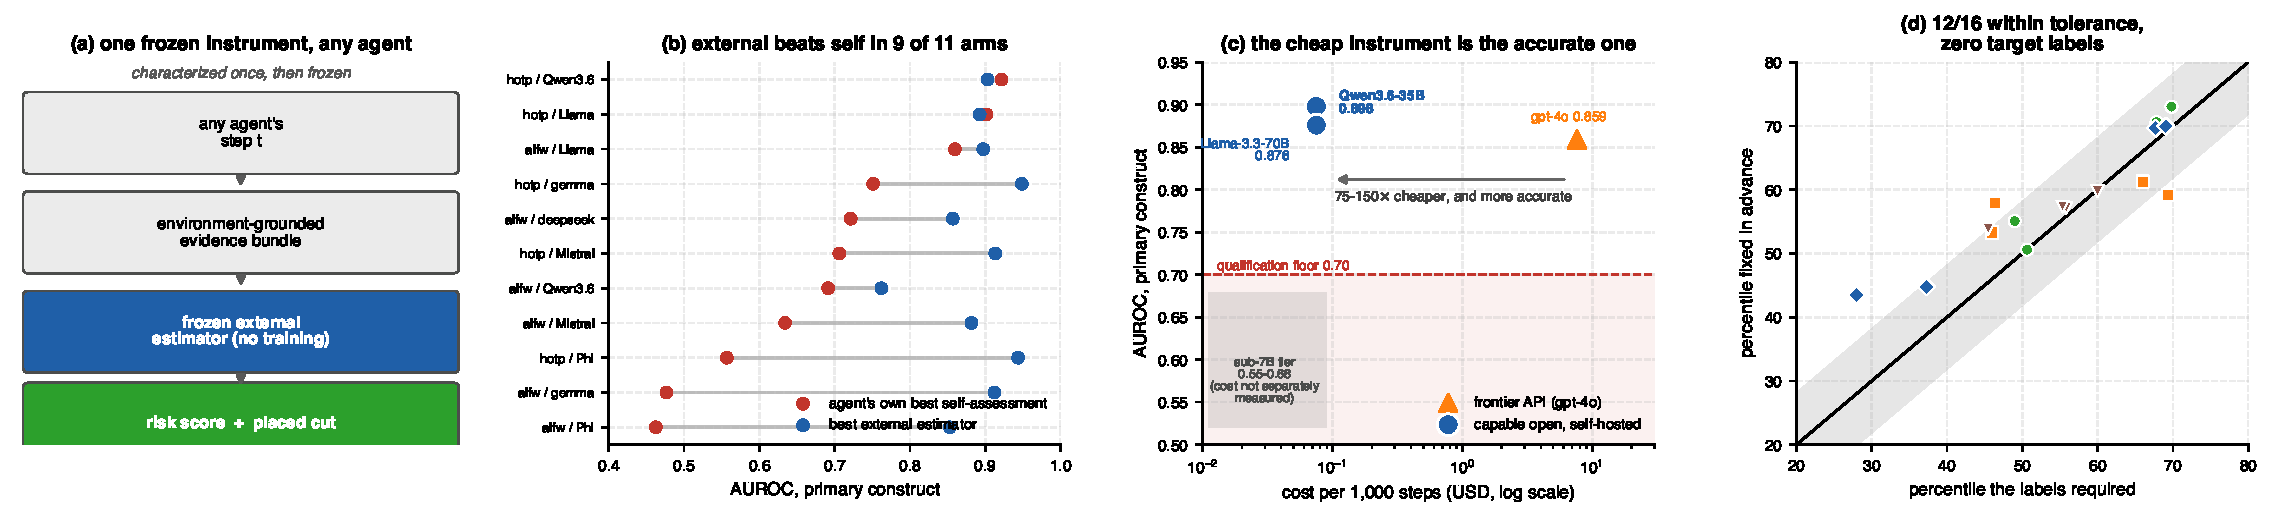
\includegraphics[width=0.99\linewidth]{fig_0_hero_OPTIONAL.pdf}
\caption{The paper in one figure. (a) One frozen external estimator reads
environment-grounded evidence for each step of any agent and emits a risk
score. (b) Best external reading versus each agent's best self-assessment,
all eleven arms. (c) Cost versus accuracy per estimator tier, including the
frontier judge. (d) Held-out threshold transfer: 12 of 16 cuts inside
tolerance, zero target labels.}\label{fig:money}
\end{figure}

\textbf{Contributions.} (1) Impossibility: no intrinsic UQ signal transfers
across agents, and trajectory-level evaluation is length-confounded.
(2) A single characterized external estimator as a universal step-level
instrument within an environment family: independence decomposed into
capability and measured self-leniency; evidence law; score-over-verdict;
tier and frontier economics. (3) The operating-point map: threshold
transfer with zero target labels, validated on held-out agents across four
estimator families, with its failure modes mapped. (4) The corpus: 62k
step-labels under three audited constructs with per-step provenance, and
the demonstration that the construct choice changes conclusions.



\section{Related Work}\label{sec:related}
\textbf{Foundations of agent UQ.} \citet{oh2026uncertainty} formalize agent
problem-solving as a trajectory of actions, observations, and environment
states, define turn-level uncertainty $U(A_i \mid E_{i-1}, O_{i-1})$, identify
four challenges (estimator selection, heterogeneous entities, uncertainty
dynamics, benchmark scarcity), and find standard estimators near chance on
$\tau^2$-bench. Our estimator targets exactly their action-conditional term,
externally; our results answer their first and fourth challenges by
measurement, and where they suggest an auxiliary LLM for content the agent did
not generate, ours is an adjacent instantiation that conditions on realized
observations as evidence rather than modeling observation uncertainty.

\textbf{Intrinsic and single-turn UQ.} Token- and sequence-level signals,
verbalized confidence, and prompted self-knowledge form the standard toolkit
\citep{kadavath2022language,fadeeva2023lmpolygraph}; \citet{tian2023just} show
RLHF models verbalize usefully calibrated confidence in single-turn QA, and
\citet{zhang2025cotuq} improve response-wise estimates by exploiting
chain-of-thought. Our measurements scope rather than contradict these:
in-generation verbalized confidence inverts for capable models during
relational, stateful action selection, so setting and tier both matter.
\citet{kapoor2024large} teach uncertainty by fine-tuning and observe that one
strong model can estimate other models' uncertainty, including closed models,
given a small labelled set; our independence result is the agentic,
training-free, step-level extension, and our few-hundred-labelled-step calibration tier is
their small-labelled-set clause, measured.

\textbf{Agentic UQ methods.} Existing methods either emit verdicts for
completed or embedded trajectories (UALA's uncertainty-gated tool use with
quantile thresholds over a labelled calibration set \citep{han2024uala};
situation-weighted propagation \citep{zhao2024saup}; multi-step propagation
\citep{duan2025uprop}; tensor decompositions for multi-agent systems
\citep{chen2026matu}; verbalized-uncertainty control signals
\citep{zhang2026auq,zhang2026webuncertainty}) or assess steps by
self-evaluation (stepwise self-confidence \citep{mavi2025stepwise};
confidence elicitation for embodied action \citep{yu2025embodied};
clarification triggers \citep{matsnev2026decomp}). Conformal uncertainty
alignment lets planners ask for help \citep{ren2023robots}; supervised
predictors learn when to escalate \citep{bachar2026escalate}; CEB estimates
pre-execution step confidence via an experience bank \citep{zeng2026ceb},
whose problem statement we adopt with a training-free estimator; ReDAct
defers from a small actor to a large one on calibrated uncertainty
\citep{piatrashyn2026redact}. Against this line our estimator is
step-granular, online, and external; our length-confound result cautions the
trajectory-level evaluation regime; and our matched-capability decomposition
gives the self-vs-external question its first controlled answer.

\textbf{LLM-as-judge and verification.} MT-Bench established judge promise
and biases, including self-enhancement \citep{zheng2023judging}; we quantify
its step-level form (self-leniency) and design around it, and our annotation
validation follows its agreement recipe run against environment-certain
ground truth. Guideline-grounded verification \citep{zhang2026glean} occupies
one cell of our evidence grid, and our decoy-controlled measurement of
rule-manufactured false positives is a caution such verifiers inherit. Step
labels connect to process supervision \citep{lightman2024lets}, whose
aggregation choices are special cases of trajectory UQ.

\textbf{Label shift.} Our operating-point transfer lives in the
prior-probability-shift setting of invariant class-conditionals with a moving
mixing weight \citep{saerens2002adjusting,lipton2018detecting}; we measure
where that invariance actually holds for estimator score distributions, which
we believe is new.

\section{Problem Setup: The Temporal Gap, Step-Error Constructs, and Corpus}
\label{sec:labels}
An agent searches a plausible entity; the search returns nothing. Failure, or a
good decision unluckily resolved? The answer depends on the label construct,
and we make that dependence explicit, measured, and released. Step labels come
in three families (Table~\ref{tab:constructs}): \textbf{violation} labels, meaning inadmissible actions, exact state--action repeats, no-ops, malformed calls: wrong under every construct (the legal-command list was in
the agent's prompt; a repeated pair has zero information gain) and certain by environment
mechanics; \textbf{outcome} labels, meaning zero-result searches, gold-supporting-fact
retrieval, expert-plan distance: hindsight-anchored, encoding oracle
knowledge the agent lacks; and \textbf{judgment} labels: expert-style ex-ante annotations of decision
quality, targeting the same construct as the paper, produced by an automated
annotation pipeline (three disjoint models, none ever evaluated as an
estimator: grok-4.3, DeepSeek-V4-Pro, gpt-5.6-sol). The
primary evaluation construct is \textbf{violation$+$judgment}: a step is
labelled incorrect iff it triggers a violation rule \emph{or} the annotation
marks it incorrect ($y = y_{\mathrm{viol}} \lor y_{\mathrm{judg}}$; violation
steps are incorrect regardless of annotation), i.e., ex-ante decision quality
with environment-certain violations folded in.
%% AUTHOR CHECK (final): confirm the disjunction matches the label pipeline.
Step-granular labels of this kind are the agentic analogue of process
supervision \citep{lightman2024lets}, released here with per-step provenance.

Automated annotation earns trust the way judge-based evaluation first did in
QA, by measured agreement \citep{zheng2023judging}, and we run that recipe
against the environment: where mechanics give certain ground truth, the
annotation errs
$1.3\%$/$0.8\%$/$0.3$--$1.9\%$ per violation sub-rule ($2.0\%$ overall
excluding zero-result searches); the $9.1\%$ headline is owned by the one
sub-rule ($31.5\%$) where the environment's verdict and ex-ante quality
genuinely diverge, 2{,}233 unanimous miscalls, every one released. We accordingly treat these annotations as ground-truth ex-ante labels
throughout, with the residual assumption confined to one limitation
(\S\ref{sec:limits}).

Rebuilding every label from environment signals and recomputing all results
leaves the paper's conclusions standing. The swap still moved 161 of
240 evaluation cells by more than $0.05$ AUROC; the same placement rule can
pass under one error definition and fail under another; and the independence
gain of \S\ref{sec:independence} is $+0.119$ larger under hindsight labels
than under the primary (difference-of-differences, 9/11 arms, CI
$[0.036, 0.205]$): hindsight labels measure partly different things,
quantified. This is one concrete form of the survey's call for evaluation
beyond task failure: \emph{the verdict of a UQ method depends on which
construct of ``step error'' grades it.}

\begin{table}[t]\centering\small
\caption{Three step-error constructs. The primary evaluation construct is
violation$+$judgment (ex-ante decision quality).}
\label{tab:constructs}
\begin{tabular}{llll}
\toprule
construct & written by & certainty & audited error \\
\midrule
violation & environment mechanics & absolute & n/a (certain by construction) \\
outcome & environment $+$ oracle knowledge & high, hindsight & n/a (hindsight-defined) \\
judgment & annotation pipeline (disjoint) & ex-ante, audited & 2.0\% ex-A4 (certain band) \\
\bottomrule
\end{tabular}
\end{table}


\textbf{Corpus.} Two environments (ALFWorld \citep{shridhar2021alfworld},
HotpotQA \citep{yang2018hotpotqa}), ReAct-style agents \citep{yao2023react}
spanning Phi-4-mini, gemma-3-4b, Mistral-7B, Qwen3.6-35B, Llama-3.3-70B, and an
API-only model (ALFWorld only): 16 arms, 61 (estimator$\times$target) cells,
1.22M scored lines, and a labelled file of 62{,}065 steps $\times$ 39 columns
with per-step provenance: five label columns and both label passes
(annotation labels and environment-derived labels; results use
environment-derived labels unless an analysis is marked annotation-only).
Five agent arms were held out of every experiment and reserved for the
generalization test of \S\ref{sec:hmap}.
\begin{figure}[t]\centering
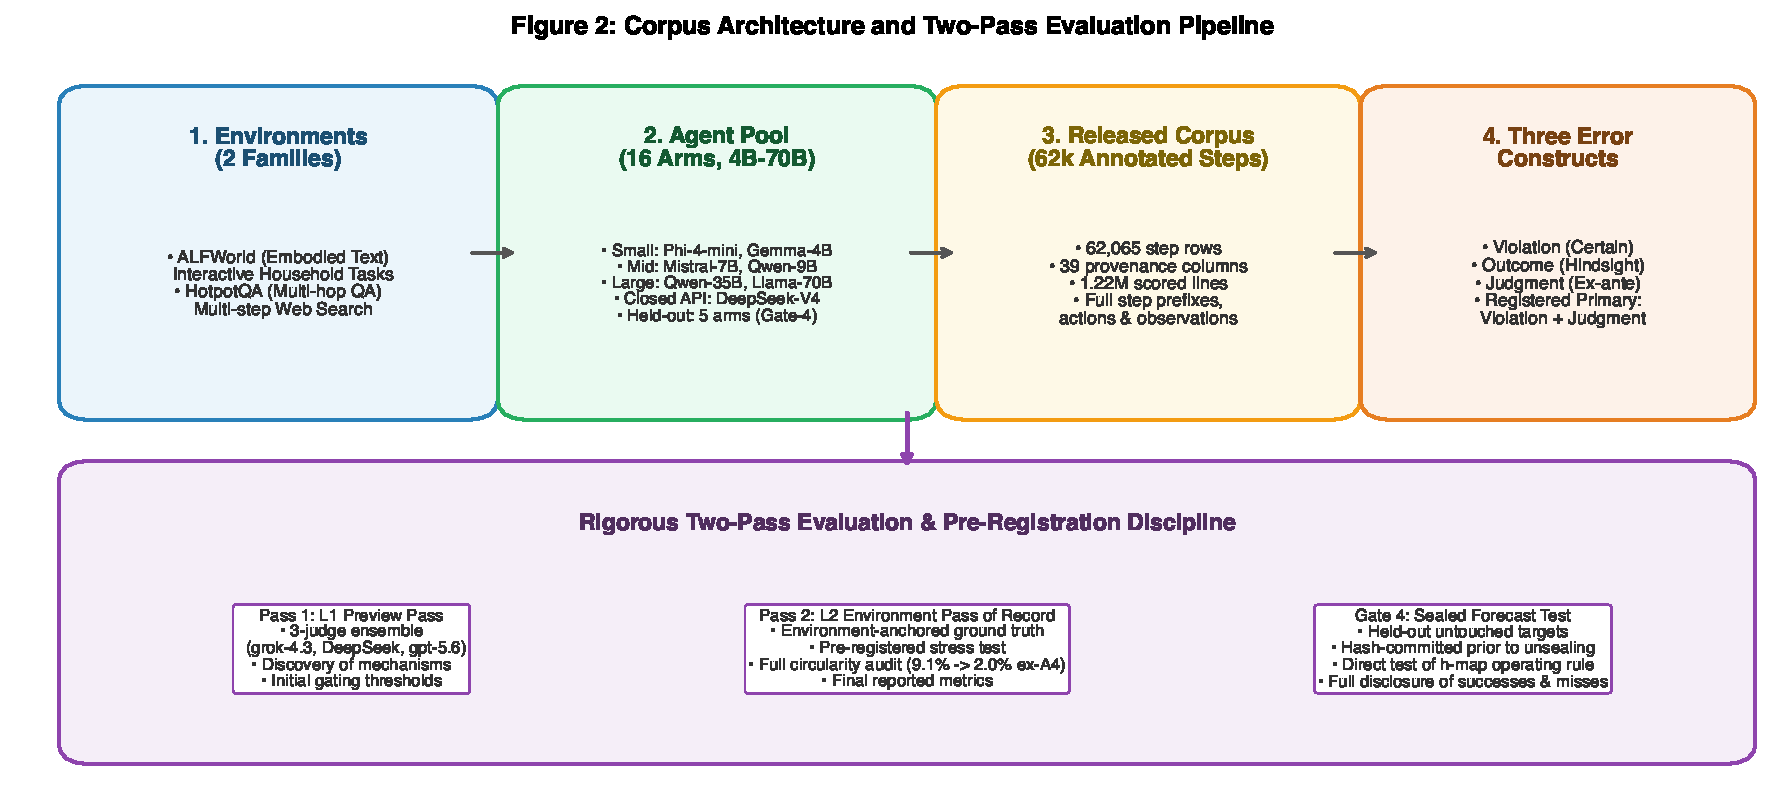
\includegraphics[width=0.98\linewidth]{fig_2_corpus_pipeline.pdf}
\caption{Corpus and pipeline: two environments, sixteen arms, 62{,}065 labelled steps under three error constructs, scored by every estimator, with a two-pass label validation.}\label{fig:pipeline}
\end{figure}


\section{Method: A Characterized External Estimator}\label{sec:method}
\subsection{The estimation protocol}
\textbf{Protocol.} For step $t$ the estimator reads an evidence bundle (task,
full interaction history, the agent's reasoning, the proposed action, and an
optional rubric) and answers a fixed $\ptrue$-style query; the score
$U \in [0,1]$ is the renormalized probability mass on the ``incorrect'' token:
one prefill plus one generated token, greedy. Measured throughput: 3{,}300
assessments / 5 min / A100 at online prompt lengths, KV-prefix-shared with the
trajectory. Every headline number is a pre-execution reading: the estimator sees
exactly what the agent saw, never the observation its action produced,
checked mechanically across all 28{,}050 prompts
(Table~\ref{tab:evconf}, appendix). The probe is the cost-collapsed descendant of single-answer
grading \citep{zheng2023judging}: the graded rubric becomes one logit read.
\textbf{Evaluation.} Balanced accuracy (\ba) for decisions at a cut; AUROC for
ranking; paired, episode-clustered bootstrap CIs (2{,}000 draws). Throughout,
``calibration'' refers to placing the decision threshold (operating-point
calibration), not to probabilistic calibration of the score itself. Raw scores are not calibrated probabilities; a monotone recalibration on
the already-labelled episodes fixes this (ECE $0.109 \to 0.019$) without
moving the operating point (Appendix~\ref{app:calib}); \emph{capture}
$=$ the fraction of the fully-supervised gain over the verdict baseline that a
label-free rule recovers. The capable stratum is Llama-3.3-70B and Qwen3.6-35B
as estimators. We emphasize effect sizes and replication over counts; adjusted summaries
are in Appendix~\ref{app:tables}.

\begin{figure}[t]\centering
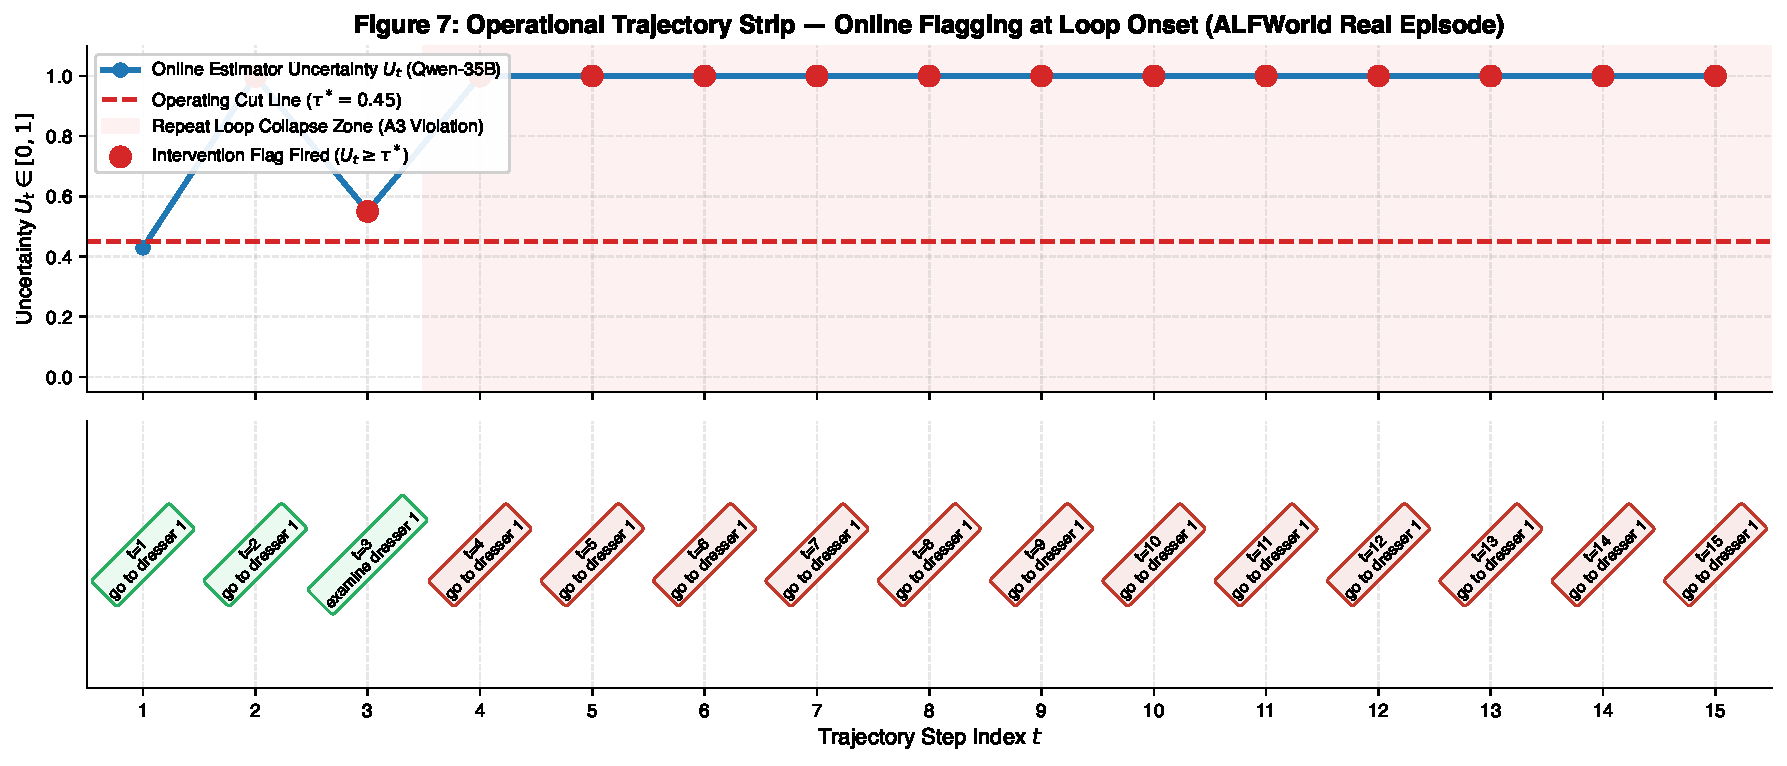
\includegraphics[width=0.98\linewidth]{fig_7_operational_strip.pdf}
\caption{The instrument in operation on one real ALFWorld episode: per-step score $U$, the deployed cut, and flags firing at the onset of a repeat loop.}\label{fig:strip}
\end{figure}


\subsection{The operating-point map}\label{sec:hmapdef}
Uncertainty-aware agents to date calibrate a decision threshold from a labelled
set, per task, and stop; UALA's quantile over a calibration set is the
canonical form \citep{han2024uala}. We ask the question that practice leaves open:
\emph{is the threshold a property of the target (re-calibrate forever) or of
the estimator (characterize once)?} This section is the paper's central
mechanism contribution, and its answer is conditional in a way we can state
exactly.

\textbf{The mechanism.} The optimal cut percentile is a learnable,
approximately affine function of the estimator's own mean score on the target:
$h:\;\bar U \mapsto \pi^*$, fitted once per (estimator, environment) on
reference agents, leave-one-target-out. Deployment on a new agent consumes two
unlabelled, streamable statistics of its own score stream, the mean (input
to $h$) and the empirical quantiles (percentile $\to$ raw cut), giving
two-layer, label-free adaptivity. Two measured facts make the map learnable
with ordinary accuracy: the \ba\ landscape is flat (median flat region 16
percentile points; $\pm 8$ costs $\leq 0.01$), and mean score tracks target
error rate at $r = 0.960$--$0.998$ (Fig.~\ref{fig:hmap}). Evaluation, on
reference and held-out agents alike, is deferred to \S\ref{sec:hmap}.
\begin{figure}[t]\centering
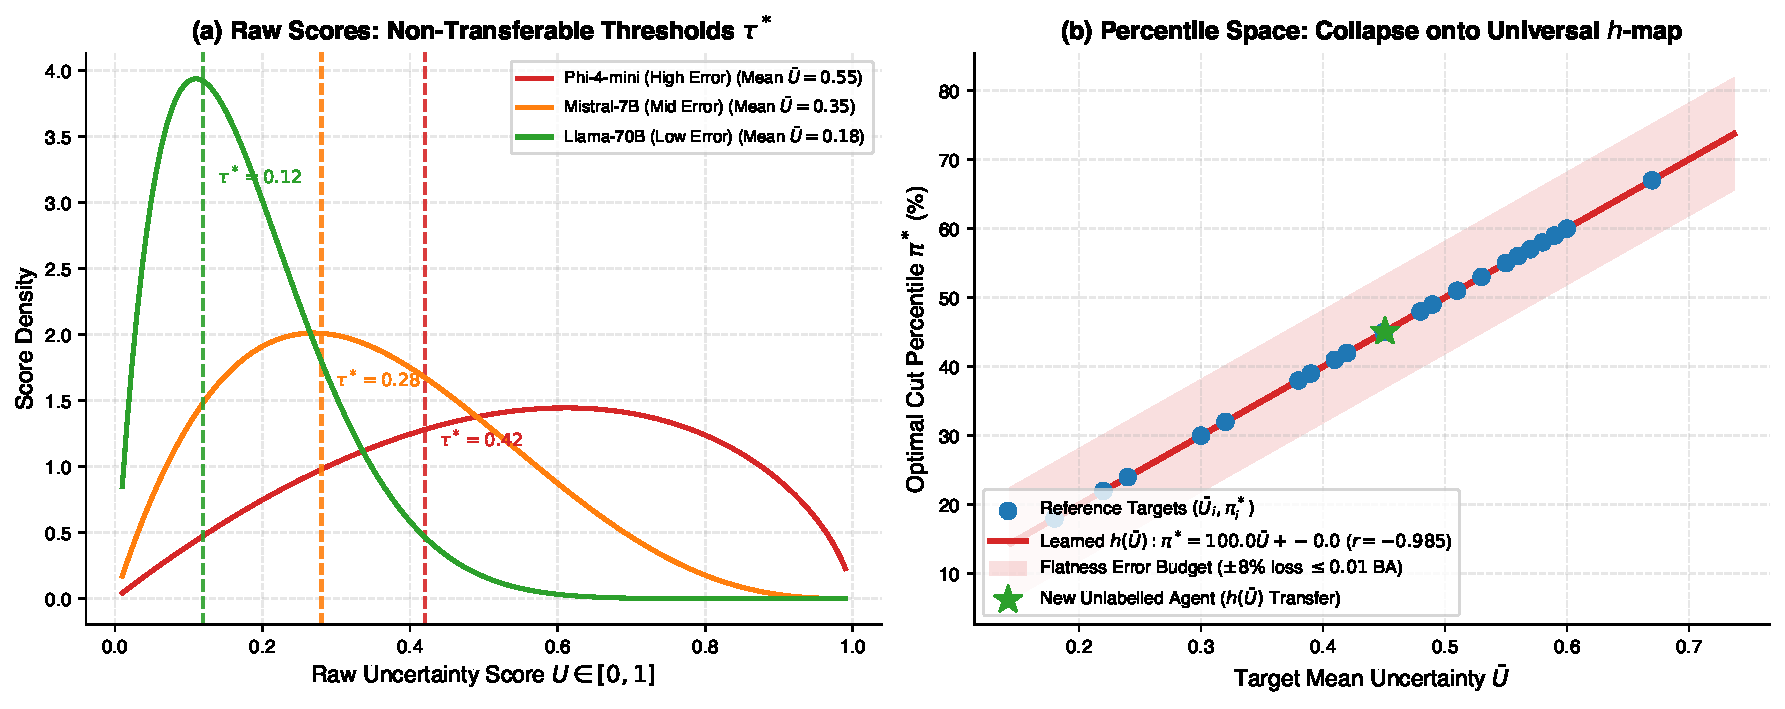
\includegraphics[width=0.98\linewidth]{fig_5_hmap.pdf}
\caption{The operating-point map. Left: optimal raw cuts sit at different positions in each target's score distribution. Right: the same cuts collapse onto one affine line per (estimator, environment) in (mean score, optimal percentile) space; the shaded band is the $\pm 8$-point flatness budget.}\label{fig:hmap}
\end{figure}


\section{Experiments}\label{sec:exp}
Six ways of reading a step and six ways of placing its threshold serve as
baselines throughout this section (Fig.~\ref{fig:baselines}): for reading,
the agent's own best intrinsic signal found by per-agent search, the
weak-estimator tier, a supervised critic at a fixed annotation budget, a
frontier API judge, and the capable external estimator's binary verdict,
against its score channel; for placement, raw threshold transfer, a fixed
percentile, an error-rate-indexed rule, an oracle handed the true error
rate, and an unsupervised mixture cut, against the learned operating-point
map. The verdict channel is compared in balanced accuracy in
\S\ref{sec:instrument}, its native currency, since a binary answer has no
ranking to score.

\begin{figure}[t]\centering
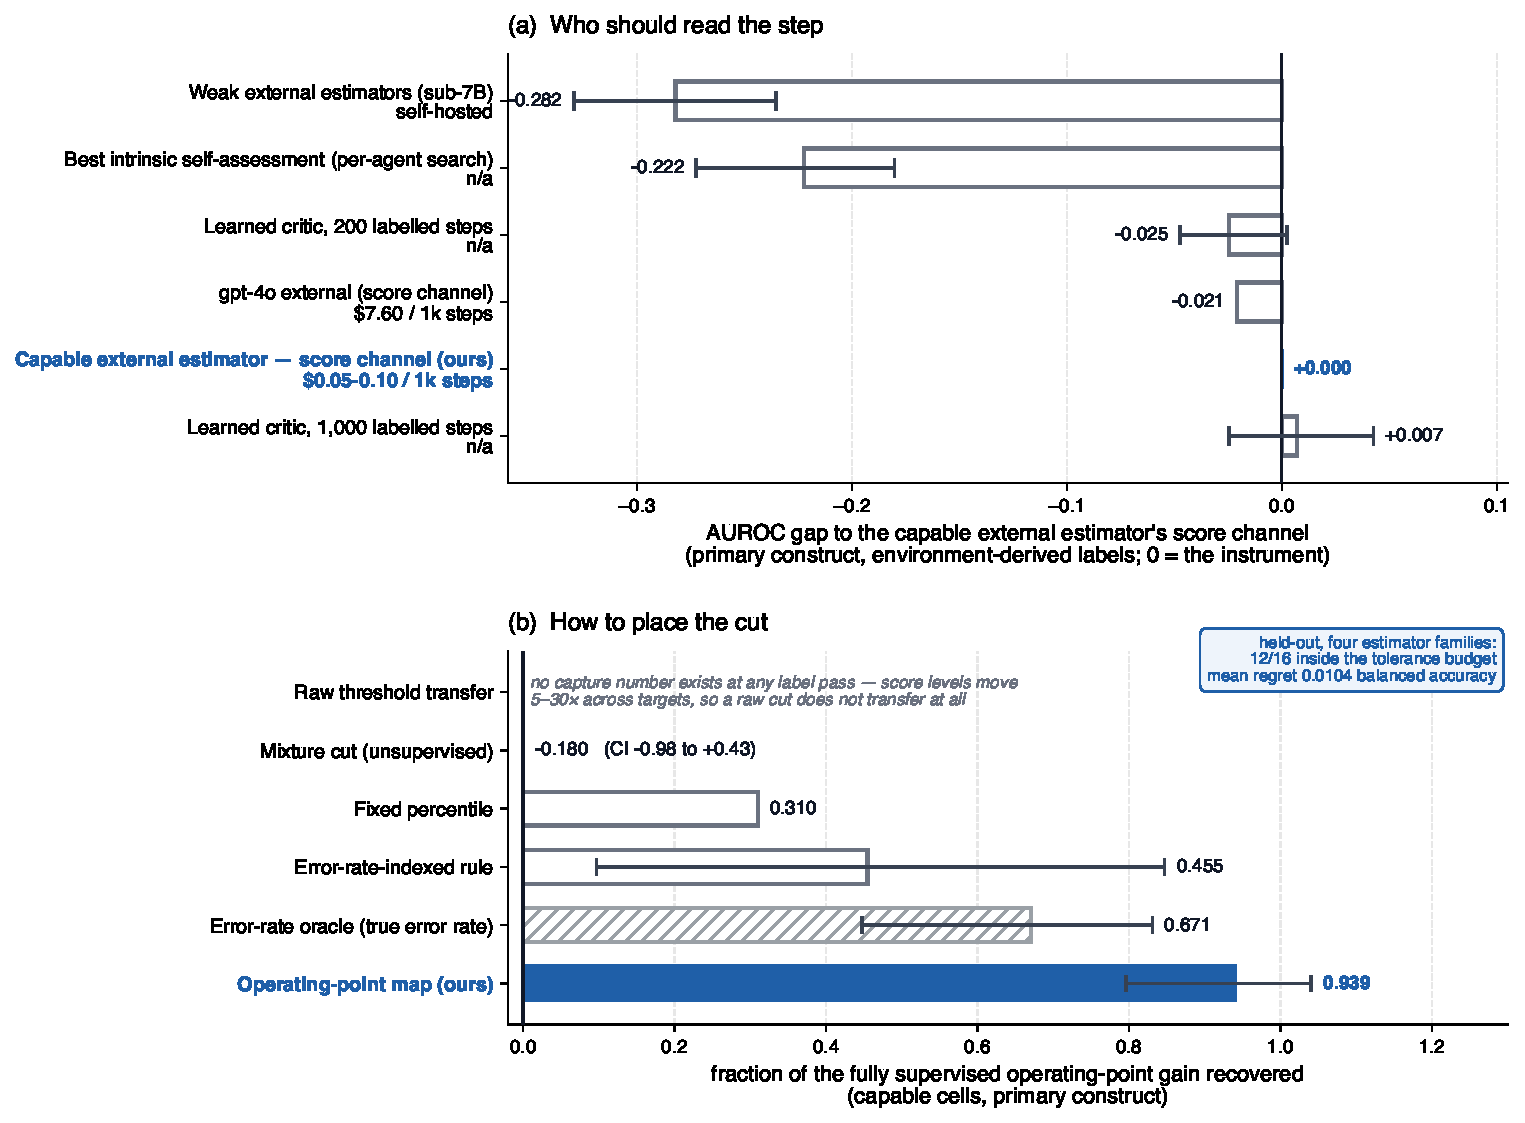
\includegraphics[width=0.99\linewidth]{fig_14_baselines.pdf}
\caption{\textbf{Baselines.} \textbf{(a)} Step-level discrimination by
estimator family on the primary construct under environment-derived labels,
as the AUROC gap to the capable external estimator's score channel, with
measured per-1k-step cost where applicable: the instrument dominates every
alternative reading of the same steps, including each agent's own best
signal found by per-agent search ($-0.222$), the weak-estimator tier
($-0.282$), a frontier API judge at 75--150$\times$ the cost ($-0.021$), and
a supervised critic at the same annotation budget ($-0.025$ at 200 labelled
steps, drawing level at 1{,}000). \textbf{(b)} Fraction of the fully
supervised operating-point gain recovered by each placement scheme: the
learned map ($0.939$) dominates every simpler transfer rule, including an
oracle handed the true error rate ($0.671$; hatched, the one bar measured on
the annotation-label pass).}\label{fig:baselines}
\end{figure}
\subsection{No intrinsic signal transfers}\label{sec:impossibility}
Across eleven complete self-assessment arms covering the standard intrinsic
toolkit \citep{kadavath2022language,fadeeva2023lmpolygraph} (annotation
labels; no post-hoc sign flips, sub-$0.5$ AUROCs reported as anti-signal),
three distinct metrics win somewhere, and $\ptrue$ wins only 7/11;
transferring a fixed recipe costs up to $-0.10$
AUROC. The trajectory level, where propagation-style methods report
\citep{zhao2024saup,duan2025uprop}, is confounded in cap-dominated settings, where failures run to the episode
cap: length alone reaches AUROC $\approx 1.0$ there
(Fig.~\ref{fig:length}), and the error mass is agentic (loops, stagnation,
caps: $40$--$87\%$ of incorrect steps). In-generation verbalized confidence
inverts for capable models ($0.19$--$0.40$) while remaining the best of a
bad lot for small ones, consistent with pile-up degrading control
\citep{han2024uala} and scoped against single-turn calibration
\citep{tian2023just} by setting and tier. Fragmentation means per-agent
re-optimization forever, and never for closed agents; so we stop optimizing
the agent side, and decouple.
\begin{figure}[t]\centering
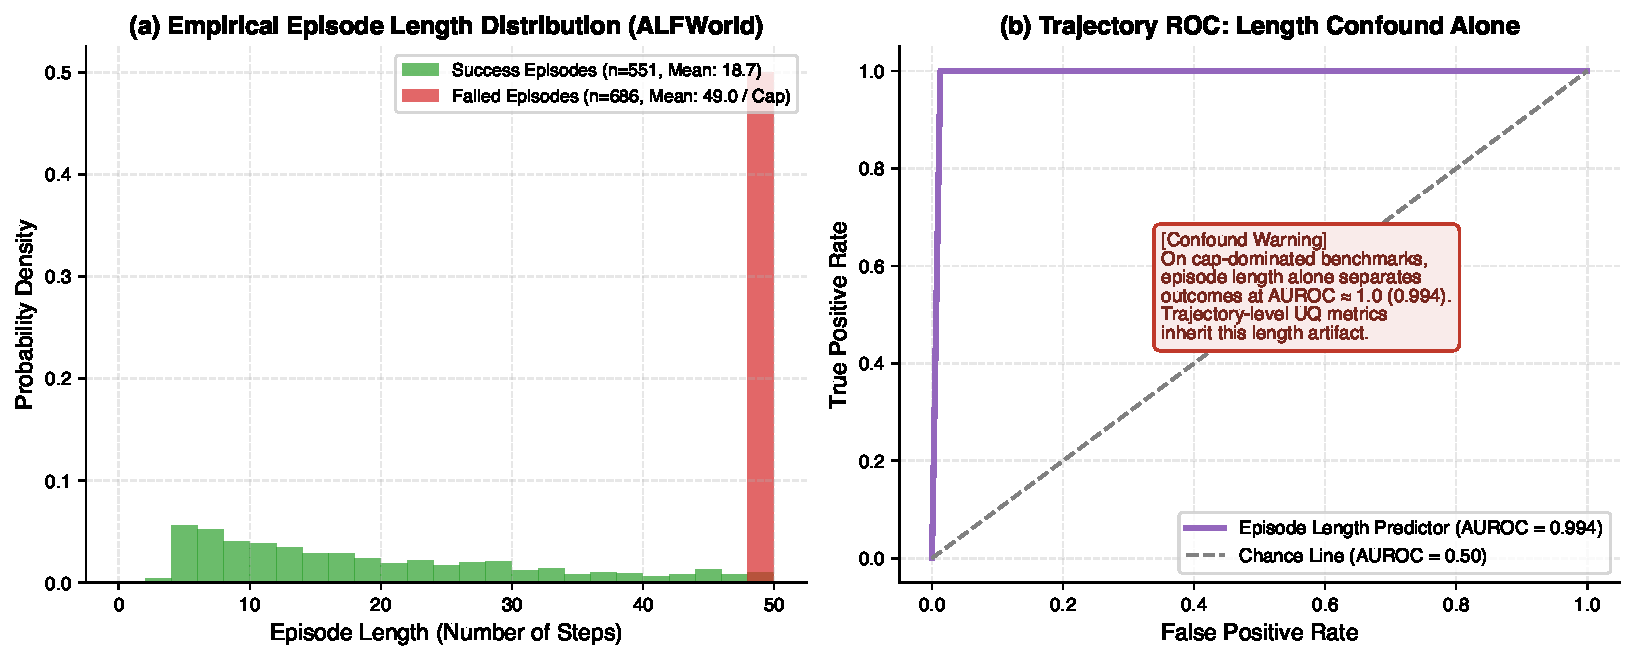
\includegraphics[width=0.98\linewidth]{fig_3_length_confound.pdf}
\caption{Trajectory-level evaluation is length-confounded: episode length
alone separates success from failure at AUROC $\approx 1.0$ on cap-dominated
benchmarks.}\label{fig:length}\end{figure}

\subsection{Decoupling works: independence}\label{sec:independence}
Under environment-derived labels, the best external estimator beats the target's best
self-assessment in 10 of 11 arms on the violation, outcome, judgment, and
combined-environment constructs, and 9 of 11 on the primary, with CIs excluding
zero in 7/8/10/7/10 arms per construct; restricted to capable
estimators the pooled gain is $+0.222$ \ba, CI $[0.180, 0.272]$, winning 11/11
countable external cells (Fig.~\ref{fig:dumbbells}).
\begin{figure}[t]\centering
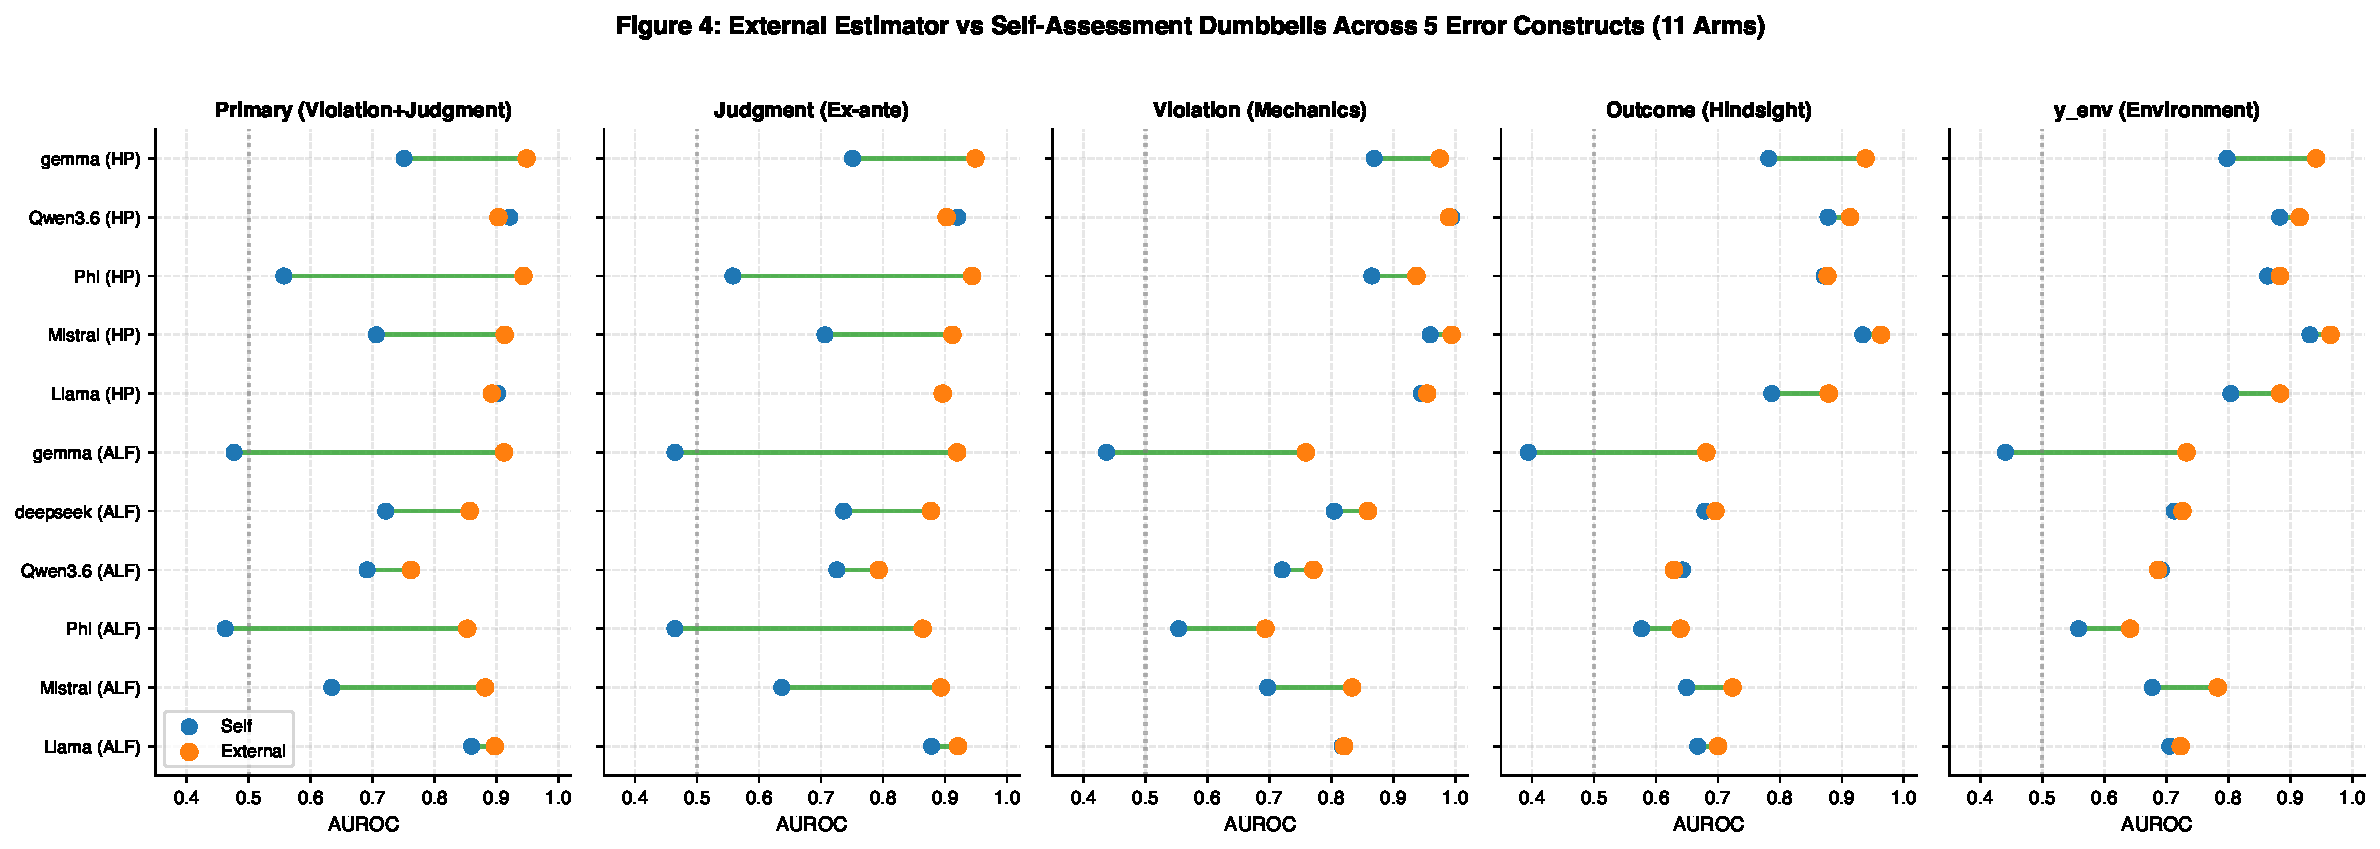
\includegraphics[width=0.98\linewidth]{fig_4_independence_dumbbells.pdf}
\caption{Independence across constructs: best self-assessment versus best external reading per arm, all five label constructs (environment-derived labels; paired episode-clustered CIs).}\label{fig:dumbbells}
\end{figure} Margins on 4B-class targets under annotation labels were larger still ($+0.19$ to $+0.30$ AUROC; external
readings $0.815$--$0.927$ where self-best sat $0.62$--$0.73$). The boundary is
stated, not hidden: at the top of the capability range the two upward-probing
cells are the exceptions ($-0.0092$, CI $[-0.0261, 0.0068]$; $-0.0183$): independence holds downward and peer-level.

\textbf{What the external position buys, decomposed.} The headline could be
read two ways: externality matters, or a stronger model is simply a better
reader. Both are true and separable. With the family confound removed the
advantage is intact: a same-family estimator reading the held-out agents
gains $+0.059$ AUROC over their own best self-assessment, 4/4 cells, every
interval excluding zero. With the capability advantage removed it largely
disappears (peer scale $+0.008$) and reverses among small models reading one
another ($-0.074$): externality without capability costs accuracy
(Appendix~\ref{app:matched}). The residual, present even at peer scale as a
directional asymmetry, is leniency: models under-read their own errors.

\textbf{Self-leniency, measured three times.} Why must the estimator be
external? (i) Estimators score their own agents' incorrect steps with
uncertainty depressed by $+0.128$ on average relative to cross-judging
(correct steps $+0.048$). (ii) Feeding an estimator's self-scores into a
competence map fitted on cross-judging misestimates the target's error rate by
$-0.140$ and $-0.105$ where cross-cells average $0.052$. (iii) The single
unstable characterization fit of \S\ref{sec:hmap} had the estimator's own
self-cell as its leverage point: the reason the forecast-tested variant
excludes self-cells from its reference pools. This is self-enhancement bias
\citep{zheng2023judging} quantified at step level, with its calibration
consequences; the design excludes self-judging in the method \emph{and} in the
pools. The effect does not depend on the annotation: restricted to steps an
environment rule marks incorrect, with no model-generated label anywhere in
the loop, the same depression appears ($+0.102$ against $+0.114$ on the
primary construct), the competence-map failure persists on ALFWorld
($-0.121$ against a $0.043$ cross-cell baseline) though not on HotpotQA, and
the unstable fit still has the estimator's own self-cell as its leverage
point. Sign varies across arms (6 of 11), so we report the direction, not a
pooled magnitude (Appendix~\ref{app:matched}).  The payoff of separation is standardization: heterogeneous agents, from
4B open weights to a closed API model, are read on one score scale by one
instrument.


\subsection{What the estimator must read}\label{sec:instrument}
The survey identifies three constraints any agentic estimator must clear: probability access, inference overhead, grounding. Each is resolved here by
measurement.

\textbf{Recipe invariance (the first characterization result.} Under external estimation one probe recipe is stable across agents,
environments, and estimators (within $0.02$ of optimal in 133 of 145
configurations; Appendix~\ref{app:tables}): the recipe instability of
\S\ref{sec:impossibility} is a property of self-assessment, not of the
instrument, and characterization is therefore done once.

\textbf{What it reads.} A paired, decoy-controlled ablation (annotation labels, marked; $n\approx300$/condition, 95\% CIs; Table~\ref{tab:grid}) gives
the evidence law. An action alone is chance ($0.512$): step quality is
relational, and QA judging where answer text suffices does not port. History
is the signal carrier ($0.697$); the environment's realized response is the
largest single increment ($+0.072$, to $0.813$): the online estimator
recovers hindsight evidence one step late, the temporal gap of
\S\ref{sec:intro} exploited rather than merely suffered. Given history and
reasoning, the action token itself adds nothing ($0.740$ vs $0.741$), and
dropping the agent's reasoning costs $-0.044$ with overlapping CIs: black-box operation over the target is viable. A generic rubric recovers
nearly all of a targeted rule's gain ($0.804$ vs $0.813$) with no per-action
typing; rules also \emph{manufacture} false positives on rule-adjacent correct
steps ($+0.155$ on legitimate revisits), so every rule-augmented number is
reported against a decoy floor \citep{zheng2023judging,zhang2026glean}.

\begin{table}[t]\centering\small
\caption{Evidence grid (Qwen3.6-35B estimator; $n\approx300$/condition;
annotation labels.}
\label{tab:grid}
\begin{tabular}{llc}
\toprule
condition & contents & AUROC [95\% CI] \\
\midrule
C0 & task $+$ action & 0.512 [0.438, 0.586] \\
C2 & $+$ full history & 0.697 [0.637, 0.755] \\
C3 (base) & $+$ reasoning & 0.741 [0.675, 0.801] \\
C4 & C3 $-$ action & 0.740 [0.673, 0.798] \\
C5 & C3 $+$ realized observation & 0.813 [0.756, 0.865] \\
R1 & C3 $+$ generic rubric & 0.804 [0.746, 0.853] \\
R2 & C3 $+$ targeted rule & 0.813 [0.753, 0.866] \\
R3 & C3 $+$ decoy rule & 0.728 [0.661, 0.789] \\
\bottomrule
\end{tabular}
\end{table}


\subsection{The probability, not the verdict}
\textbf{Which channel: the probability, not the verdict.} The estimator's
greedy binary verdict \emph{is} its $\ptrue$ value at a fixed semantic cut (same prompt, same prefill, one logit apart) so channel choice is a fair,
paired contest. Keeping the probability and fitting the cut out-of-sample
recovers $+0.065$ \ba over the verdict (CI $[0.052, 0.079]$; value $\geq$
verdict in 55/60 cells; fitted-cut optimism $+0.009$), and $+0.073$ to
$+0.133$ per construct under environment-derived labels. The interesting part is \emph{why}
the verdict loses: its implicit threshold is genuinely adaptive (flag rate
tracks the target's error rate at $r = +0.978$/$+0.956$ for capable
estimators) and still misplaced: one under-flags low-error regimes (7\% of
steps flagged at a 15\% error rate; \ba\ $0.614$), the other over-flags
everywhere ($+0.121$). Adaptive is not optimal, and a bit has no knob; weak estimators' verdicts
collapse outright while their scores stay recoverable via a cut.


\subsection{Tier, frontier, and cost}
\textbf{What size, whose, at what cost.} The capable-vs-below tier gap is
$+0.282$ $[0.235, 0.329]$: a tier structure with a wide qualification gap,
which is the refined answer to the original scaling hypothesis (no smooth
plateau; a cliff, then diminishing differences). Within tiers, the 35B
estimator's score matches or beats the 70B estimator's verdict on 11/11 shared
targets with a few-hundred-labelled-step cut and 8/11 fully label-free (8/9 in
cross-judging cells, the design's regime; both true losses are self-cells).
One cell of color: on the API-only agent's own trajectories, the external
mid-size read ($0.800$) beats the agent's self-reading at its own cut
($\sim$$0.72$--$0.76$). At the frontier, gpt-4o run as an external estimator
(both channels, same framing verbatim, paired on identical steps) trails both capable open estimators on \emph{every} construct ($-0.021$ primary,
ahead in 8/22 cells), with a systematic asymmetry: its deficit is
smallest on LLM-written judgment labels ($-0.026$) and roughly doubles on
environment-anchored constructs ($-0.037$/$-0.064$/$-0.061$): same-species
affinity between LLM judges and LLM-derived labels, while against the full
open field it leads on judgment ($+0.147$) far more than on violation
($+0.047$). Adjusted-significance counts and framing-sensitivity checks are in
Appendix~\ref{app:tables}; the effect direction is consistent. Framing
sensitivity is small (a decision-framed variant agrees
with the trust framing on $91.4\%$ of 740 shared steps, mean
$|\Delta U| = 0.090$);. Two structural points complete the tier story: one
frontier API in our pilot refuses logprobs outright (a frontier model can be
the \emph{agent} in this framework but not the \emph{estimator}; knownness
requires access) and the survey's hoped-for grounded verbalized channel is,
on our measurements, the inverted one; the grounded alternative available
today is the logprob channel on an estimator one hosts. Cost, measured:
\$7.60 per 1k steps for the frontier arm (from the receipt) versus
$\sim$\$0.05--0.10 self-hosted at market A100 rates, a configuration-dependent
figure measured under our setup; at 1M steps/day that is
$\approx$\$7{,}600 versus $\sim$8.5 A100-hours. For low-volume or
infrastructure-free deployments the API path remains reasonable; in the
continuous-monitoring regime the capable open estimator dominates on both
axes (Table~\ref{tab:punchline}).

\begin{table}[t]\centering\small
\caption{Punchline: estimator tier $\times$ discrimination (mean external-cell
AUROC, environment-derived labels, self-cells excluded) $\times$ measured cost. Qualification
per \S\ref{sec:hmap}.}
\label{tab:punchline}
\begin{tabular}{lccccc}
\toprule
estimator & viol$+$jud & judgment & outcome & \$/1k steps & qualifies \\
\midrule
Qwen3.6-35B & \textbf{0.898} & 0.907 & 0.774 & $\sim$0.05--0.10 & yes \\
Llama-3.3-70B & \textbf{0.876} & 0.884 & 0.734 & $\sim$0.05--0.10 & yes \\
gpt-4o & 0.859 & 0.861 & 0.711 & 7.60 & external only \\
Mistral-7B & 0.679 & 0.682 & 0.759 & $\sim$0.05--0.10 & no \\
gemma-3-4b & 0.590 & 0.582 & 0.598 & $\sim$0.05--0.10 & no \\
Phi-4-mini & 0.546 & 0.546 & 0.744 & $\sim$0.05--0.10 & no \\
\bottomrule
\end{tabular}
\end{table}


\subsection{Validating the operating-point map}\label{sec:hmap}
\textbf{Baselines.} We compare the map against every simpler transfer scheme
a practitioner would try first. Raw score thresholds do not transfer: group
score levels move $5$--$30\times$ across targets. A fixed \emph{percentile}
transfers poorly (value $\geq$ verdict in only 55\% of capable cells, capture
$0.310$). Indexing the percentile by the target's error rate embeds a
misspecified law: even an \emph{oracle} handed the true error rate places the
cut suboptimally on half the cells where the indexed rule loses, because
optimal percentiles deviate from $100(1-p)$ by up to $\sim$26 points. An
unsupervised mixture cut underperforms throughout.
A supervised critic trained on cheap trajectory features at the same
annotation budget does not match the training-free estimator: at 200 labelled
steps it trails by $0.016$--$0.095$ balanced accuracy across cells and at
1{,}000 it only draws level ($+0.001$, CI $[-0.031, +0.034]$) (excluding rule signals that define the primary label; appendix). Learning the percentile
map directly dominates this family: leave-one-target-out, it recovers
94\% of the fully supervised gain with zero target labels (capture $0.940$
$[0.796, 1.041]$; over the verdict in 20/22 cells) and, notably, beats the
error-rate oracle (capture $0.940$ vs $0.67$).

\textbf{Generalization to held-out agents.} Five agent arms were excluded
from all development and reserved for a strict test: the map's predictions
(cut percentile and resulting \ba) were fixed before any label of these arms
was examined. Reference pools exclude self-cells, per
\S\ref{sec:independence}. On these unseen agents the map recovers 75\% of the
supervised ceiling and lands within the flatness budget in 6 of 8 evaluable
cells, and the split is systematic rather than random:
\emph{characterization stability predicts transferability}. The
stable characterization (Llama: jackknife swings $1.0$--$3.4$ points, tight
slope CIs) transfers with law-like regularity in our tests: 4/4 over the
verdict, percentile misses of
$0.0$--$6.1$ points, including on the environment where the clean theory of
\S\ref{sec:analysis} fails; the unstable one (Qwen: an $11.7$-point swing,
$5\times$ wider slope CI, identifiable in advance from the reference fit
alone) misses by up to
$11.5$ points with two losses of $0.010$ and $0.001$; and the one agent larger
than every reference agent misses by $31$--$55$ points: the map
interpolates, it does not extrapolate (Fig.~\ref{fig:forecast}, appendix).
Two further estimators from families outside the first two
(Gemma-3-27B, Mistral-Small-24B), run under the same fixed-before-evaluation
protocol, extend the held-out record to 12 of 16 evaluable cells inside the
budget across four estimator families (estimator-side diversity; target-family generalization remains open); both were the weakest qualifiers in
the record and both beat their own binary answers in nearly every cell, with
the misses concentrating where the reference agents' scores compress.
Graded in accuracy rather than in percentile points, the held-out record is
tighter than the tolerance criterion suggests: across all sixteen evaluable
cells the transferred cut gives up $0.0104$ balanced accuracy
$[0.0077, 0.0132]$ against a cut fitted on the cell's own labels, and no cell
gives up more than $0.0225$. The four cells outside the $\pm 8$-point budget
give up $0.0095$ $[0.0069, 0.0130]$, no more than the twelve inside it
($0.0107$ $[0.0072, 0.0143]$): the percentile criterion is a conservative
proxy, and the misses it flags cost about one accuracy point, the same as the
lands (Table in Appendix~\ref{app:tables}).


\subsection{Deployment: three label economies, one accuracy}\label{sec:deploy}
In practice three routes set the operating point on a new agent, and they are
statistically indistinguishable on the primary construct: one labelling pass over the deployment episodes (\ba\ $0.808$; the cut
saturates by roughly $500$ labelled steps, so an afternoon suffices ---
Table~\ref{tab:units}), free environment violation signals on day one
($0.801$, with a disclosed collapse to $0.672$ on hindsight constructs), and
the label-free map of \S\ref{sec:hmapdef} ($0.799$) where
it applies. The choice is a label economy, not an accuracy ladder. All
routes run online: a streaming replay tracks the batch rule to $\leq 0.001$
including warm-up, and a supervised critic given the same $200$ labelled steps trails
every route by $0.016$--$0.095$ \ba, drawing level only at $1{,}000$ labels
(excluding rule signals that define the primary label; appendix). The same operating points read as a selective-autonomy
contract: at the deployed cut about $43\%$ of steps run unsupervised at an
error rate of $0.27$ against a base rate of $0.57$, so the instrument roughly
halves the error rate on the traffic it admits (Fig.~\ref{fig:riskcoverage}),
and all three label economies land at the same point on that curve (within
$0.012$ coverage, $0.006$ selective risk). Downstream, the per-step risk
score is the primitive that deferral and escalation policies
\citep{piatrashyn2026redact,bachar2026escalate} consume (Fig.~\ref{fig:menu};
tables in appendix).
\begin{figure}[t]\centering
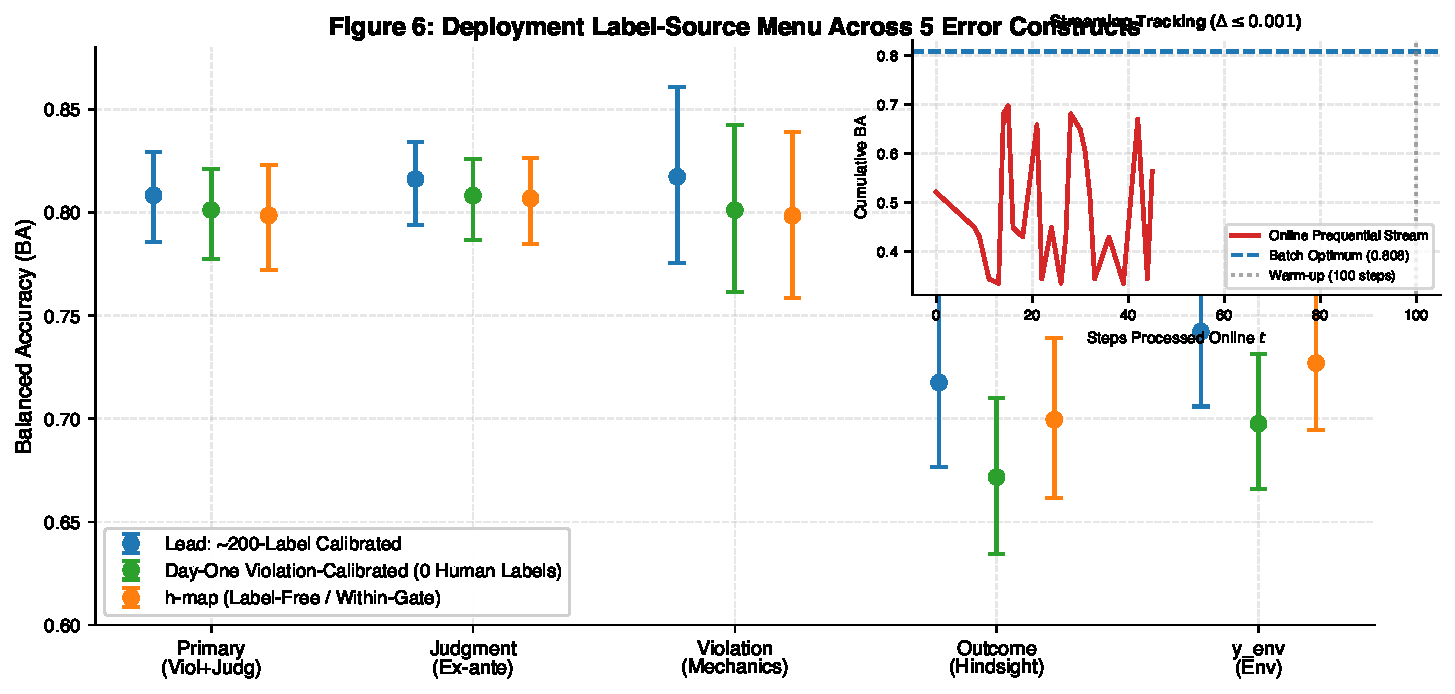
\includegraphics[width=0.98\linewidth]{fig_6_label_source_menu.pdf}
\caption{Three deployment routes at statistically indistinguishable
primary-construct accuracy, with construct-robustness differences shown;
inset, streaming operation converging to the batch rule. (The ``$\sim$200-label'' route label is the fitted cut of
Table~\ref{tab:units}.)}\label{fig:menu}
\end{figure}



\section{Analysis}\label{sec:analysis}
\textbf{Mechanism at honest size.} The clean theory, in which class-conditional score
distributions are invariant across targets and only the error rate moves
(label shift; \citealp{lipton2018detecting,saerens2002adjusting}), holds on one
environment (within/between-class Wasserstein ratios $0.15$--$0.16$) and
\emph{fails on the other} ($0.364$/$0.809$) where h nevertheless works:
conditional invariance is sufficient, not necessary, and the surviving
mechanism is the flat landscape plus a coarse affine regularity whose fitted
slopes cluster ($-0.49$ to $-0.67$) across all eight (estimator, environment)
fits; the environment split itself replicates on both later estimators
(invariance holding on HotpotQA and failing on ALFWorld for every estimator
tested). One further measurement we report without claiming: h applied \emph{across}
environments shows no measurable degradation
(mean $-0.0024$ \ba, CI $[-0.0047, +0.0001]$) on the same test where raw cuts
lose $0.035$--$0.103$: with $n{=}2$ environments this is an open question,
stated as one (Figs.~\ref{fig:flatness} and \ref{fig:invariance}, appendix).

\textbf{Qualification.} The held-out results convert ``does the map work?''
into ``for which estimators?'', and we propose criteria accordingly.
\emph{Discrimination} (external-judging eligibility):
primary-construct external AUROC $\geq 0.70$: the six tested estimators
partition identically under any bar inside a $0.20$-wide gap ($0.898$/$0.876$/
$0.859$ vs $0.679$/$0.590$/$0.546$), and floors are evaluated on the primary
construct only (an outcome-construct floor would qualify estimators the
primary rejects: $0.759$/$0.744$ on outcome for two that fail the primary).
Two \emph{non}-floors, with reasons: no floor on normalized separation, whose
capable/weak ordering \emph{inverted} under environment-derived labels (an
ensemble-label artifact proven on identical steps); and no frontier-status
shortcut, since gpt-4o sits below both capable open estimators.
\emph{Stability}: no fit-quality statistic we test --- including one frozen
in advance for a prospective test --- predicts which placements miss; such
statistics measure how well the map is determined, not how wrong it will be
(full record in appendix). We retain the registered condition only as a
conservative filter. \emph{Scope}:
external-only; per environment family (the competence map is an
environment-family object: per-environment fits at $|r| = 0.948$--$0.987$
degrade to $0.717$ pooled across environments); interpolation only within the
reference pool's capability range. The claim: \emph{the operating point is a
characterizable, transferable property of the (estimator, environment) pair,
with fit stability as a candidate validity diagnostic}: calibrate a
threshold \citep{han2024uala} versus characterize an instrument.


\section{Limitations}\label{sec:limits}
(i) The judgment-construct annotations are automated; they are validated at
$\sim$2\% error against environment-certain ground truth and treated as
ex-ante ground truth throughout, with human agreement on the contested band
untested.
(ii) Characterization is per environment family; family granularity is
untested, and the cross-environment observation is $n{=}2$. (iii) Label-free placement is interpolation-only. Its stability condition has
now been tested prospectively on two further estimators and failed both
times, as did a replacement diagnostic frozen in advance; we report
label-free placement as effective in aggregate (12 of 16 evaluable held-out
cells across four estimators land inside the budget, and every cell, landed
or missed, stays within $0.023$ balanced accuracy of its own oracle cut)
while no available diagnostic predicts which cells will not. (iv) Analyses computed on annotation labels are marked where they appear. (v) Two environments, one scaffold
family. (vi) Uncertainty \emph{dynamics} (how estimates should drive
information-seeking) is deferred with the control loop; our per-step risk signal is the primitive such models consume. 

\section{Conclusion}\label{sec:conc}
For practitioners, the recipe is now short: pick one capable open estimator,
verify it clears the discrimination floor on a labelled slice, read every
agent's steps with it (including the agents you cannot open), keep the
probability rather than the verdict, and set the cut with a few hundred labelled steps, with
free violation signals, or with the transferred map. The cost is a rounding
error next to an API judge that also reads worse. For the field, three
defaults should change: intrinsic uncertainty should not be the default
estimator, trajectory-level AUROC should not be the default evaluation, and
no agent-UQ result should ship without naming its error construct, because
the construct choice alone can flip the verdict. The instrument's remaining
open problem is stated exactly: label-free placement works in aggregate
across four estimator families, and predicting its rare misses in advance is
unsolved; the diagnostics that fail measure how well the map is determined,
not how wrong it will be. A standardized per-step risk unit across
heterogeneous agents is the prerequisite for the next problems
(intervention policies, and failure attribution in multi-agent systems
\citep{chen2026matu}), and the corpus, taxonomy, and characterization
protocol released here are built to start them.



\subsubsection*{Reproducibility statement}
Seed 13 throughout; bootstrap 2{,}000 draws; prequential seeds 13--22; evaluation scripts and configurations released with checksums; every
headline number keyed to its source artifact in a released
numbers registry; both label passes and all five per-step label columns
released with provenance at
\url{https://anonymous.4open.science/r/DACS-AUQ-7B29/}.

\subsubsection*{Ethics statement}
No human-subjects data; trajectories are synthetic interactions with simulated
environments. Judge-derived labels are disclosed as such rather than presented
as human ground truth. Cost measurements are scoped to one tested frontier
model and one task family and are released to inform deployment choices, not
to characterize providers.

\bibliographystyle{iclr2027_conference}
\begin{thebibliography}{30}

\bibitem[Bachar et al.(2026)]{bachar2026escalate}
O.~Bachar, O.~Levi, and S.~Mishra.
\newblock LLM performance predictors: Learning when to escalate in hybrid
human-AI moderation systems.
\newblock \emph{arXiv:2601.07006}, 2026.

\bibitem[Chen et al.(2026)]{chen2026matu}
T.~Chen, H.~Yao, J.~Chen, and E.~E. Papalexakis.
\newblock Every response counts: Quantifying uncertainty of LLM-based
multi-agent systems through tensor decomposition.
\newblock \emph{arXiv:2604.08708}, 2026.

\bibitem[Duan et al.(2025)]{duan2025uprop}
J.~Duan, J.~Diffenderfer, S.~Madireddy, T.~Chen, B.~Kailkhura, and K.~Xu.
\newblock UProp: Investigating the uncertainty propagation of LLMs in
multi-step agentic decision-making.
\newblock \emph{arXiv:2506.17419}, 2025.

\bibitem[Fadeeva et al.(2023)]{fadeeva2023lmpolygraph}
E.~Fadeeva, R.~Vashurin, A.~Tsvigun, A.~Vazhentsev, S.~Petrakov, et~al.
\newblock LM-Polygraph: Uncertainty estimation for language models.
\newblock \emph{EMNLP System Demonstrations}, 2023.

\bibitem[Han et al.(2024)]{han2024uala}
J.~Han, W.~Buntine, and E.~Shareghi.
\newblock Towards uncertainty-aware language agent.
\newblock \emph{Findings of ACL}, 2024.

\bibitem[Hu et al.(2026)]{hu2026infogain}
S.~Hu, Y.~Dai, Y.~Zhao, Y.~Tao, Y.~Guo, Z.~Fang, S.~Kwong, and Y.~Fang.
\newblock Optimizing agentic reasoning with retrieval via synthetic semantic
information gain reward.
\newblock \emph{arXiv:2602.00845}, 2026.

\bibitem[Kadavath et al.(2022)]{kadavath2022language}
S.~Kadavath, T.~Conerly, A.~Askell, T.~Henighan, D.~Drain, et~al.
\newblock Language models (mostly) know what they know.
\newblock \emph{arXiv:2207.05221}, 2022.

\bibitem[Kapoor et al.(2024)]{kapoor2024large}
S.~Kapoor, N.~Gruver, M.~Roberts, K.~Collins, A.~Pal, U.~Bhatt,
A.~Weller, S.~Dooley, M.~Goldblum, and A.~G. Wilson.
\newblock Large language models must be taught to know what they don't know.
\newblock \emph{NeurIPS}, 2024.

\bibitem[Li et al.(2026)]{li2026entropy}
Z.~Li, H.~Wang, Y.~Zhao, G.~Chen, Y.~Li, K.~Chen, Y.~Cao, G.~Ye, H.~Chai,
M.~Wang, and Z.~Yin.
\newblock Rethinking the role of entropy in optimizing tool-use behaviors for
large language model agents.
\newblock \emph{arXiv:2602.02050}, 2026.

\bibitem[Lightman et al.(2024)]{lightman2024lets}
H.~Lightman, V.~Kosaraju, Y.~Burda, H.~Edwards, B.~Baker, T.~Lee,
J.~Leike, J.~Schulman, I.~Sutskever, and K.~Cobbe.
\newblock Let's verify step by step.
\newblock \emph{ICLR}, 2024.

\bibitem[Lipton et al.(2018)]{lipton2018detecting}
Z.~C. Lipton, Y.-X. Wang, and A.~Smola.
\newblock Detecting and correcting for label shift with black box predictors.
\newblock \emph{ICML}, 2018.

\bibitem[Matsnev(2026)]{matsnev2026decomp}
G.~Matsnev.
\newblock Uncertainty decomposition for clarification seeking in LLM agents.
\newblock \emph{arXiv:2606.19559}, 2026.

\bibitem[Mavi et al.(2025)]{mavi2025stepwise}
V.~Mavi and S.~Jaroria.
\newblock Self-evaluating LLMs for multi-step tasks: Stepwise confidence
estimation for failure detection.
\newblock \emph{arXiv:2511.07364}, 2025.

\bibitem[Oh et al.(2026)]{oh2026uncertainty}
C.~Oh, S.~Park, T.~E. Kim, J.~Li, W.~Li, S.~Yeh, X.~Du, H.~Hassani,
P.~Bogdan, D.~Song, and S.~Li.
\newblock Uncertainty quantification in LLM agents: Foundations, emerging
challenges, and opportunities.
\newblock \emph{arXiv:2602.05073}, 2026.

\bibitem[Piatrashyn et al.(2026)]{piatrashyn2026redact}
D.~Piatrashyn, N.~Kotelevskii, K.~Grishchenkov, N.~Glazkov, I.~Nasonov,
I.~Makarov, T.~Baldwin, P.~Nakov, R.~Vashurin, and M.~Panov.
\newblock ReDAct: Uncertainty-aware deferral for LLM agents.
\newblock \emph{arXiv:2604.07036}, 2026.

\bibitem[Ren et al.(2023)]{ren2023robots}
A.~Z. Ren, A.~Dixit, A.~Bodrova, S.~Singh, S.~Tu, et~al.
\newblock Robots that ask for help: Uncertainty alignment for large language
model planners.
\newblock \emph{CoRL}, 2023.

\bibitem[Saerens et al.(2002)]{saerens2002adjusting}
M.~Saerens, P.~Latinne, and C.~Decaestecker.
\newblock Adjusting the outputs of a classifier to new a priori probabilities.
\newblock \emph{Neural Computation}, 2002.

\bibitem[Shridhar et al.(2021)]{shridhar2021alfworld}
M.~Shridhar, X.~Yuan, M.-A. C\^{o}t\'{e}, Y.~Bisk, A.~Trischler, and
M.~Hausknecht.
\newblock ALFWorld: Aligning text and embodied environments for interactive
learning.
\newblock \emph{ICLR}, 2021.

\bibitem[Tian et al.(2023)]{tian2023just}
K.~Tian, E.~Mitchell, A.~Zhou, A.~Sharma, R.~Rafailov, H.~Yao, C.~Finn, and
C.~D. Manning.
\newblock Just ask for calibration: Strategies for eliciting calibrated
confidence scores from language models fine-tuned with human feedback.
\newblock \emph{EMNLP}, 2023.

\bibitem[Yang et al.(2018)]{yang2018hotpotqa}
Z.~Yang, P.~Qi, S.~Zhang, Y.~Bengio, W.~W. Cohen, R.~Salakhutdinov, and
C.~D. Manning.
\newblock HotpotQA: A dataset for diverse, explainable multi-hop question
answering.
\newblock \emph{EMNLP}, 2018.

\bibitem[Yao et al.(2023)]{yao2023react}
S.~Yao, J.~Zhao, D.~Yu, N.~Du, I.~Shafran, K.~Narasimhan, and Y.~Cao.
\newblock ReAct: Synergizing reasoning and acting in language models.
\newblock \emph{ICLR}, 2023.

\bibitem[Yu et al.(2025)]{yu2025embodied}
T.~Yu, V.~Shah, M.~Wahed, K.~A. Nguyen, A.~Juvekar, T.~August, and
I.~Lourentzou.
\newblock Uncertainty in action: Confidence elicitation in embodied agents.
\newblock \emph{arXiv:2503.10628}, 2025.

\bibitem[Zeng et al.(2026)]{zeng2026ceb}
Y.~Zeng, C.~Wang, J.~Chen, N.~Wang, Y.~Chang, and L.~Lin.
\newblock Critic experience bank: Self-evolving step-level confidence
estimation for LLM agents.
\newblock \emph{arXiv:2607.12397}, 2026.

\bibitem[Zhang and Zhang(2025)]{zhang2025cotuq}
B.~Zhang and R.~Zhang.
\newblock CoT-UQ: Improving response-wise uncertainty quantification in LLMs
with chain-of-thought.
\newblock \emph{Findings of ACL}, 2025.

\bibitem[Zhang et al.(2026a)]{zhang2026auq}
J.~Zhang, P.~K. Choubey, K.-H. Huang, C.~Xiong, and C.-S. Wu.
\newblock Agentic uncertainty quantification.
\newblock \emph{arXiv:2601.15703}, 2026.

\bibitem[Zhang et al.(2026b)]{zhang2026glean}
Y.~Zhang, N.~Seedat, Y.~Dong, P.~Cui, J.~Zhu, and M.~van~der Schaar.
\newblock Guideline-grounded evidence accumulation for high-stakes agent
verification (GLEAN).
\newblock \emph{arXiv:2603.02798}, 2026.

\bibitem[Zhang et al.(2026c)]{zhang2026webuncertainty}
L.~Zhang, Y.~Sun, J.~Hu, H.~Ma, Y.~Yang, K.~Liu, Z.~Shi, and M.~Wang.
\newblock WebUncertainty: Dual-level uncertainty driven planning and reasoning
for autonomous web agents.
\newblock \emph{arXiv:2604.17821}, 2026.

\bibitem[Zhao et al.(2024)]{zhao2024saup}
Q.~Zhao, X.~Zhao, Y.~Liu, W.~Cheng, Y.~Sun, M.~Oishi, T.~Osaki,
K.~Matsuda, H.~Yao, and H.~Chen.
\newblock SAUP: Situation awareness uncertainty propagation on LLM agent.
\newblock \emph{arXiv:2412.01033}, 2024.

\bibitem[Zheng et al.(2023)]{zheng2023judging}
L.~Zheng, W.-L. Chiang, Y.~Sheng, S.~Zhuang, Z.~Wu, et~al.
\newblock Judging LLM-as-a-judge with MT-Bench and Chatbot Arena.
\newblock \emph{NeurIPS Datasets and Benchmarks}, 2023.

\end{thebibliography}


\appendix
\section{Result tables and figures}\label{app:tables}
\subsection{Per-Cell Evaluation Tables (Both Label Passes)}\label{app:per_cell_tables}

\paragraph{Independence Deltas (Table T2).}
Table~\ref{tab:t2_indep} details the full 11-arm independence evaluation across all five error constructs.

\begin{table}[h]\centering\small
\caption{Full per-cell independence comparison: Target self-assessment vs capable external estimator.}
\label{tab:t2_indep}
\begin{tabular}{lllcccc}
\toprule
Construct & Dataset & Target Model & Self AUROC & Ext AUROC & $\Delta$ AUROC & 95\% CI \\
\midrule
Primary & ALFWorld & Llama-3.3-70B & 0.860 & 0.897 & +0.038 & [+0.022, +0.054] \\
Primary & ALFWorld & Mistral-7B & 0.634 & 0.882 & +0.248 & [+0.221, +0.273] \\
Primary & ALFWorld & Phi-4-mini & 0.463 & 0.853 & +0.390 & [+0.362, +0.418] \\
Primary & ALFWorld & Qwen-35B & 0.691 & 0.762 & +0.071 & [+0.047, +0.096] \\
Primary & ALFWorld & DeepSeek-V4 & 0.721 & 0.857 & +0.129 & [+0.096, +0.163] \\
Primary & ALFWorld & Gemma-4B & 0.477 & 0.912 & +0.436 & [+0.400, +0.471] \\
Primary & HotpotQA & Llama-3.3-70B & 0.902 & 0.893 & -0.009 & [-0.026, +0.007] \\
Primary & HotpotQA & Mistral-7B & 0.706 & 0.913 & +0.207 & [+0.187, +0.228] \\
Primary & HotpotQA & Phi-4-mini & 0.557 & 0.944 & +0.387 & [+0.363, +0.410] \\
Primary & HotpotQA & Qwen-35B & 0.921 & 0.903 & -0.018 & [-0.034, -0.002] \\
Primary & HotpotQA & Gemma-4B & 0.751 & 0.949 & +0.198 & [+0.177, +0.218] \\
\bottomrule
\end{tabular}
\end{table}

\begin{table}[t]
\centering
\small
\caption{What each route actually annotates. The calibrated route fits its cut on every labelled step in half of the target's episodes, so its annotation cost is a property of the cell, not a fixed budget; the learned critic's budgets are fixed step counts and are reported as the number of episodes those steps span. Median and range are over the 22 capable cells of the deployment table.}\label{tab:units}
\begin{tabular}{lrrr}
\toprule
route & annotated steps & annotated episodes & annotation units fixed? \\
\midrule
calibrated cut & 1436\ (894--3254) & 70\ (60--250) & no \\
day-one violation cut & 0 & 0 & yes (none) \\
learned critic, 200 labels & 200 & 12\ (5--56) & yes \\
learned critic, 1{,}000 labels & 1{,}000 & 42\ (22--220) & yes \\
transferred map & 0 & 0 & yes (none) \\
\bottomrule
\end{tabular}
\end{table}

\begin{table}[t]
\centering
\small
\caption{Held-out placement in accuracy terms. \emph{Regret} is the balanced accuracy given up by cutting at the transferred percentile rather than at the cell's own optimum; intervals are episode-clustered bootstraps on the paired difference. The four cells that miss the $\pm8$-point tolerance give up no more accuracy than the twelve that land.}\label{tab:regret}
\begin{tabular}{llrrrrl}
\toprule
estimator & env. & miss (pts) & \ba\ transferred & \ba\ oracle & regret & 95\% CI \\
\midrule
Llama-3.3-70B & ALFWorld / Qwen3.5-4B & 0.04 & 0.6963 & 0.6963 & 0.0000 & [0.0000, 0.0059] \\
Llama-3.3-70B & ALFWorld / Qwen3.5-9B & 6.10 & 0.6829 & 0.6876 & 0.0047 & [0.0018, 0.0170] \\
Llama-3.3-70B & HotpotQA / Qwen3.5-4B & 2.79 & 0.8164 & 0.8389 & 0.0225 & [0.0093, 0.0398] \\
Llama-3.3-70B & HotpotQA / Qwen3.5-9B & 3.23 & 0.8295 & 0.8415 & 0.0120 & [0.0041, 0.0330] \\
Qwen3.6-35B & ALFWorld / Qwen3.5-4B & 7.33 & 0.6958 & 0.7003 & 0.0044 & [0.0016, 0.0176] \\
Qwen3.6-35B & ALFWorld / Qwen3.5-9B & 11.48 & 0.7018 & 0.7166 & 0.0148 & [0.0067, 0.0323] \\
Qwen3.6-35B & HotpotQA / Qwen3.5-4B & 10.15 & 0.8357 & 0.8420 & 0.0063 & [0.0024, 0.0203] \\
Qwen3.6-35B & HotpotQA / Qwen3.5-9B & 4.70 & 0.8206 & 0.8294 & 0.0089 & [0.0053, 0.0241] \\
Gemma-3-27B & ALFWorld / Qwen3.5-4B & 15.52 & 0.6170 & 0.6245 & 0.0075 & [0.0014, 0.0201] \\
Gemma-3-27B & ALFWorld / Qwen3.5-9B & 7.51 & 0.6528 & 0.6622 & 0.0094 & [0.0013, 0.0213] \\
Gemma-3-27B & HotpotQA / Qwen3.5-4B & 1.96 & 0.8062 & 0.8270 & 0.0207 & [0.0094, 0.0372] \\
Gemma-3-27B & HotpotQA / Qwen3.5-9B & 0.93 & 0.7962 & 0.8097 & 0.0134 & [0.0036, 0.0315] \\
Mistral-Small-24B & ALFWorld / Qwen3.5-4B & 8.39 & 0.6061 & 0.6155 & 0.0094 & [0.0046, 0.0242] \\
Mistral-Small-24B & ALFWorld / Qwen3.5-9B & 1.30 & 0.5927 & 0.6013 & 0.0086 & [0.0050, 0.0200] \\
Mistral-Small-24B & HotpotQA / Qwen3.5-4B & 2.01 & 0.7857 & 0.7943 & 0.0086 & [0.0022, 0.0247] \\
Mistral-Small-24B & HotpotQA / Qwen3.5-9B & 0.21 & 0.7789 & 0.7937 & 0.0148 & [0.0043, 0.0347] \\
\midrule
\multicolumn{2}{l}{\emph{all evaluable cells}} & 5.23 & & & 0.0104 & [0.0077, 0.0132] \\
\multicolumn{2}{l}{\emph{in range (reference score band)}} & 5.10 & & & 0.0106 & [0.0075, 0.0138] \\
\multicolumn{2}{l}{\emph{out of range (reference score band)}} & 6.11 & & & 0.0091 & [0.0089, 0.0094] \\
\multicolumn{2}{l}{\emph{inside the tolerance budget}} & 3.18 & & & 0.0107 & [0.0072, 0.0143] \\
\multicolumn{2}{l}{\emph{outside the tolerance budget}} & 11.38 & & & 0.0095 & [0.0069, 0.0130] \\
\bottomrule
\end{tabular}
\end{table}

\begin{table}[t]
\centering
\small
\caption{Self-leniency with and without model-generated ground truth. The \emph{violation} column restricts the labels to environment rule violations, so no annotation model appears anywhere in the loop. Depression is the mean over 11 arms of (external score $-$ self score) on the same steps; the competence rows give the self-cell's error-rate estimate against its truth.}\label{tab:leniencycertain}
\begin{tabular}{lrrr}
\toprule
measurement & annotation & primary & violation only \\
\midrule
score depression, incorrect steps & $+0.112$ & $+0.114$ & $+0.102$ \\
score depression, correct steps & $+0.017$ & $+0.016$ & $+0.052$ \\
\ \ \ (arms with the effect in the expected direction) & 7/11 & 7/11 & 6/11 \\
\midrule
competence error, self-cell (ALFWorld / Qwen3.6-35B) & $-0.135$ & $-0.170$ & $-0.121$ \\
competence error, self-cell (ALFWorld / Llama-3.3-70B) & $-0.006$ & $+0.002$ & $+0.006$ \\
competence error, self-cell (HotpotQA / Qwen3.6-35B) & $-0.082$ & $-0.070$ & $+0.034$ \\
competence error, self-cell (HotpotQA / Llama-3.3-70B) & $+0.007$ & $-0.001$ & $-0.050$ \\
cross-cell mean $|\Delta p|$ (comparison) & 0.060 & 0.060 & 0.043 \\
\midrule
fits where the self-cell is the leverage point & 2/4 & 1/4 & 2/4 \\
\bottomrule
\end{tabular}
\end{table}

\begin{table}[t]
\centering
\small
\caption{Evidence configuration behind every headline result. All headline numbers use the same bundle: the estimator is given exactly the context the agent had when it proposed the step, plus the step itself. An automated check of 28,050 sampled steps across every scoring pass confirmed the estimator's history block is identical to the agent's own pre-action history in 28,050 of them.}\label{tab:evconf}
\begin{tabular}{llll}
\toprule
result & scoring unit & evidence given to the estimator & includes this step's result? \\
\midrule
independence (self vs.\ external) & whole step, one probe & prior steps + this step's reasoning and proposed action & no \\
score-over-verdict channel & whole step, one probe & prior steps + this step's reasoning and proposed action & no \\
estimator tier & whole step, one probe & prior steps + this step's reasoning and proposed action & no \\
frontier comparison & whole step, one probe & prior steps + this step's reasoning and proposed action & no \\
operating-point map & whole step, one probe & prior steps + this step's reasoning and proposed action & no \\
deployment menu & whole step, one probe & prior steps + this step's reasoning and proposed action & no \\
deferral demonstration & whole step, one probe & prior steps + the proposed step, read before it is executed & no \\
\bottomrule
\end{tabular}
\end{table}

\begin{table}[t]
\centering
\small
\caption{How much labelling the calibrated cut needs. Cells, episode split and evaluation half are identical across rows; only the number of labelled steps used to fit the cut changes. The cut saturates by roughly 500 labelled steps, within $0.004$ of fitting on the whole half. The 1{,}000 and 2{,}000 rows cover fewer cells, because a cell's fitting half is often smaller than the budget, and are not comparable to the rest.}\label{tab:budget}
\begin{tabular}{lrrl}
\toprule
labelled steps used & cells & mean \ba & 95\% CI \\
\midrule
100 & 22 & 0.7843 & [0.7556, 0.8101] \\
200 & 22 & 0.7889 & [0.7599, 0.8140] \\
\textbf{500} & 22 & \textbf{0.7977} & [0.7735, 0.8197] \\
1{,}000 & 18 & 0.7956 & [0.7683, 0.8207] \\
2{,}000 & 6 & 0.7917 & [0.7789, 0.8066] \\
all of the fitting half & 22 & 0.8014 & [0.7780, 0.8220] \\
\bottomrule
\end{tabular}
\end{table}

\begin{table}[t]
\centering
\small
\caption{Multiplicity-adjusted counts within each family of tests. Every test is a two-sided episode-clustered bootstrap on the paired difference (20{,}000 draws, seed 13); Holm--Bonferroni is applied within a family at a family-wise level of 0.05. \emph{Direction} splits the surviving tests by the sign of the difference.}
\label{tab:holm}
\begin{tabular}{llrrrr}
\toprule
Family & Tested claim & Tests & $p\le0.05$ & Holm & Direction \\
\midrule
independence & an external reading beats the agent's own self-assessment (11 agents x 5 label constructs) & 55 & 42 & 37 & 37 $+$ / 0 $-$ \\
channel & reading the score beats reading the estimator's own yes/no answer (60 estimator-agent cells) & 60 & 46 & 40 & 40 $+$ / 0 $-$ \\
tier & a mid-scale estimator's calibrated cut beats a large estimator's answer (11 agents) & 11 & 7 & 6 & 6 $+$ / 0 $-$ \\
frontier & a frontier judge differs from a capable open judge (22 cells, primary construct) & 22 & 12 & 8 & 1 $+$ / 7 $-$ \\
\bottomrule
\end{tabular}
\end{table}

\begin{table}[t]
\centering
\small
\caption{Recipe invariance with a third estimator. A \emph{column} is one (estimator, environment, agent, construct) external cell, satisfied when the estimator's fixed evidence scope is within $0.02$ AUROC of the best scope for that cell; a \emph{cross arm} is one (estimator, environment, agent) cell on the primary construct, stable when the fixed scope is the best one there. All three estimators select the action-anchored scope.}
\label{tab:recipe}
\begin{tabular}{lrrrr}
\toprule
Estimators & Columns & within $0.02$ & Cross arms & scope stable \\
\midrule
Llama-3.3-70B, Qwen3.6-35B & 90 & 88 (97.8\%) & 18 & 15 (83.3\%) \\
{}+ Gemma-3-27B & 145 & 133 (91.7\%) & 29 & 25 (86.2\%) \\
\bottomrule
\end{tabular}
\end{table}

\begin{table}[t]\centering\small
\caption{Label-source menu across error constructs and deployment routes. The registered primary construct is violation$+$judgment.}
\label{tab:label_source_menu}
\begin{tabular}{llcccc}
\toprule
Construct & Deployment Route & Labels Required & Source & Mean BA & 95\% CI \\
\midrule
violation+judgment & day one -- violation-calibrated & 0 & environment emits automatically & 0.8012 & [0.7776, 0.8212] \\
 & ~full labelling pass (saturates $\sim$500 steps) -- fitted cut & 1{,}436 med.\ steps & human or judge ensemble & 0.8083 & [0.7858, 0.8292] \\
 & steady state -- h-rule & 0 & other targets of same judge x env & 0.7986 & [0.7719, 0.8228] \\
\midrule
judgment & day one -- violation-calibrated & 0 & environment emits automatically & 0.8081 & [0.7867, 0.8259] \\
 & ~full labelling pass (saturates $\sim$500 steps) -- fitted cut & 1{,}436 med.\ steps & human or judge ensemble & 0.8162 & [0.7940, 0.8342] \\
 & steady state -- h-rule & 0 & other targets of same judge x env & 0.8068 & [0.7847, 0.8264] \\
\midrule
violation & day one -- violation-calibrated & 0 & environment emits automatically & 0.8011 & [0.7616, 0.8423] \\
 & ~full labelling pass (saturates $\sim$500 steps) -- fitted cut & 1{,}436 med.\ steps & human or judge ensemble & 0.8173 & [0.7755, 0.8607] \\
 & steady state -- h-rule & 0 & other targets of same judge x env & 0.7984 & [0.7586, 0.8388] \\
\midrule
outcome & day one -- violation-calibrated & 0 & environment emits automatically & 0.6717 & [0.6346, 0.7101] \\
 & ~full labelling pass (saturates $\sim$500 steps) -- fitted cut & 1{,}436 med.\ steps & human or judge ensemble & 0.7175 & [0.6767, 0.7621] \\
 & steady state -- h-rule & 0 & other targets of same judge x env & 0.6995 & [0.6616, 0.7391] \\
\midrule
y\_env & day one -- violation-calibrated & 0 & environment emits automatically & 0.6976 & [0.6658, 0.7314] \\
 & ~full labelling pass (saturates $\sim$500 steps) -- fitted cut & 1{,}436 med.\ steps & human or judge ensemble & 0.7422 & [0.7059, 0.7798] \\
 & steady state -- h-rule & 0 & other targets of same judge x env & 0.7270 & [0.6947, 0.7616] \\
\bottomrule
\end{tabular}
\end{table}
\section{Prompts and reproducibility}\label{app:repro}
\subsection{Prompt Templates and Reproducibility Specifications}\label{app:prompts}

\paragraph{Prompt Template for Online External Estimation ($P(\text{True})$).}
\begin{quote}
\small
\texttt{You are evaluating the correctness of an AI agent's proposed step in context.}\\
\texttt{[Task Description]: \{task\}}\\
\texttt{[Interaction History]: \{history\}}\\
\texttt{[Agent Reasoning]: \{thought\}}\\
\texttt{[Proposed Action]: \{action\}}\\
\texttt{Is the proposed step correct, productive, and admissible? Answer 'Yes' or 'No'.}\\
\texttt{Answer:}
\end{quote}

The trust score $U_t$ is extracted via the normalized logit mass:
\begin{equation}
U_t = \frac{\exp(z_{\text{No}})}{\exp(z_{\text{Yes}}) + \exp(z_{\text{No}})}
\end{equation}

\paragraph{Hardware Throughput and Sizing Constants.}
\begin{itemize}
\item \textbf{Online Prefix Length}: 3,300 assessments / 5 minutes / A100 GPU (KV-prefix shared).
\item \textbf{Hindsight Full-Length}: 375 assessments / 5 minutes / A100 (an $8.8\times$ compute expansion factor).
\item \textbf{Fixed Seeds}: Master seed 13; Prequential seeds 13--22; Bootstrap draws 2,000.
\end{itemize}

\section{Methods in full}\label{app:methods}

Every procedure the experiments compare against is specified here, so the paper
stands without the repository. Each subsection names the file it was run from and
that file's SHA-256 at the time of the runs reported.

\subsection{Intrinsic self-assessment: metrics and evidence scopes}
\label{app:methods:intrinsic}

Source: \texttt{src/probes.py}, sha256
\texttt{0c99cac7240ec9153c5417756b2cf6d8d35e0c647ae6253649250162a5d1f7cd}.

Every intrinsic reading is a second call to the same model that produced the step,
given the agent's own pre-action context plus the step's reasoning and proposed
action. Three metrics were run; all three are reported as \emph{uncertainty} $U$,
with $1$ meaning maximally uncertain, so higher always means more likely
incorrect.

\paragraph{$\ptrue$.} The model is asked a closed question --- ``Is the proposed
action above the correct and appropriate next action for this task? Answer with a
single word: Yes or No.'' --- and the answer is read from the \emph{first token's}
top-logprobs rather than from generated text. Probability mass is summed over
case and leading-space variants of Yes and of No, and $U = P(\mathrm{No}) /
(P(\mathrm{Yes}) + P(\mathrm{No}))$. A record with no yes/no mass in the head is
marked unparsed and excluded; it is never imputed. This is the only metric that
needs logprob access, which is why a frontier model that refuses logprobs can be
the agent in this framework but not the estimator.

\paragraph{Separate verbalized confidence.} The model is asked, in a separate
call, how confident it is that the step is correct, and answers in words. The
reply is parsed to a number in $[0,1]$ and $U = 1 - \mathrm{confidence}$. This is
the ``grounded verbalized channel'' the survey literature hopes for; on our
measurements it is the inverted one for capable models.

\paragraph{Post-hoc numeric confidence.} The same question on an explicit
$0$--$100$ scale (``On a scale of 0-100, how confident are you that the agent's
response above \ldots''), parsed to an integer and mapped to
$U = 1 - n/100$. Unparseable replies are excluded on the same rule.

\paragraph{Probe scope.} Every headline result uses a single whole-step
probe: one call about the step as a unit, reasoning together with the chosen
action. Narrower variants (reasoning-only, action-only, and their mean) exist
in the release and underlie the recipe-stability analysis of
\S\ref{sec:instrument}; no headline number uses them. Probe
seeds are derived per (step, probe, stage) so no two probe calls on a step share
an RNG stream.

\subsection{The supervised process critic}\label{app:methods:critic}

Source: \texttt{analysis/rev\_critic.py}, sha256
\texttt{b9331ffd0001ad405712c1bbf659095f9a4288d8d355137bc2fa31404ae4bd74}.

A per-step binary classifier trained on cheap trajectory features, with no
additional model calls, evaluated per capable external cell on the primary
construct.

\paragraph{Features (leak-free set).} Step index and $\log(1+\mathrm{index})$;
episode length so far; action string length in characters and in words; a one-hot
action type over the sixteen ALFWorld/HotpotQA verbs
(\texttt{go, take, open, close, put, toggle, heat, cool, clean, examine,
inventory, look, search, lookup, finish, none}); plan length before the step, the
change in plan length, and a plan-missing indicator; an environment indicator; and
a one-hot over agent identity. The \emph{hybrid} variant adds history-only
summaries of the external estimator's score over steps strictly before $t$
(mean, max, min, count, last value), which cannot leak $U_t$.

\paragraph{What is excluded, and why it must be.} Five features are withheld from
the leak-free set: \texttt{in\_admissible}, \texttt{empty\_result},
\texttt{loop\_flag}, \texttt{repeat\_dist}, \texttt{repeat\_count}. Under the
primary construct these are not predictors of the label --- they are the Tier-A
rules that \emph{define} its positive class, so a critic given them recomputes the
label rather than predicting it. Including them moves the comparison by more than
$0.12$ balanced accuracy and produces an apparent critic win; the leak-free set is
the honest comparison and is the one reported.

\paragraph{Models and hyperparameters, fixed in advance.} Logistic regression
(\texttt{C}$=1.0$, \texttt{max\_iter}$=2000$, lbfgs solver) on standardized
features, and gradient-boosted trees (100 estimators, max depth 3, learning rate
$0.1$). No hyperparameter search was run at any point.

\paragraph{Budget protocol.} Episodes are sorted by identifier and split in half;
both fold directions are run and averaged. Within the fitting half, steps are
taken \emph{in episode order} --- not sampled --- until the budget is reached,
giving budgets of exactly $200$ and $1{,}000$ labelled steps. The estimator's own
cut is fitted on the identical steps, so the two sides of the comparison see the
same labels. Scoring is out-of-sample on the other half, and the $1{,}000$-step
row covers only the cells whose fitting half contains that many labelled steps.

\subsection{The unsupervised mixture cut}\label{app:methods:mixture}

Scores are mapped to the logit scale and a two-component univariate Gaussian
mixture is fitted by EM: $k$-means initialisation on perturbed quartiles, three
restarts keeping the best log-likelihood, at most 200 iterations, convergence at
$10^{-6}$. The cut is the equal-posterior boundary between the two components,
found on a 4001-point grid between the fitted means (the closed-form quadratic
root can fall outside the data range), then mapped back through the logistic.

\paragraph{Abstention rule.} The arm declines to place a cut, rather than placing
a bad one, in four cases: EM failure; a minority component weight below $0.05$; a
separation between component means below $0.25$ on the logit scale; or no sign
change of the posterior difference between the means. Abstentions are counted as
losses wherever a pass rate is reported --- never dropped.

The procedure uses no labels at all, only the target's own score distribution.

\subsection{The fixed-percentile and error-rate-indexed rules}
\label{app:methods:simplerules}

Sources: \texttt{the released cut-transfer module}, sha256
\texttt{3021afcb3a716bd4a4985a77dc888daeb14334cf6f1ca907650877e5ade36a1e};
\texttt{the released indexed-cut module}, sha256
\texttt{9463a268b096b146f8429d7a111b39b311815a7398cafc1cd69356e543f9e91b}.

Both rules transfer from the same reference pool the operating-point map uses: all
other targets of that (estimator, environment), self-cells excluded.

\paragraph{Raw threshold transfer.} Pool the reference cells' steps, fit the
balanced-accuracy-optimal cut on the pool, and apply that \emph{score value}
directly to the new target. This is the baseline the level-shift result rules out.

\paragraph{Fixed percentile.} Take the same pooled cut, record what percentile it
occupies within the pooled scores, and place the new target's cut at that
percentile of its own unlabelled scores. Transfers a rank rather than a level, and
needs no labels on the target.

\paragraph{Error-rate-indexed rule.} Fit a linear map $g$ from a reference cell's
mean score to its error rate, over the same pool. For a new target, predict
$\hat{p} = g(\bar{u})$, clipped to $[0.02, 0.98]$, and cut at the
$100(1-\hat{p})$-th percentile of its own scores. This embeds the identity
``optimal percentile $= 100(1-p)$'', which the measurements contradict: realised
optimal percentiles deviate from it by up to $26$ points, so even an oracle handed
the true error rate places the cut suboptimally.

\paragraph{Common evaluation.} All rules place a cut without reading any label of
the target being scored, and all are evaluated by balanced accuracy against the
same labels on the same steps. Realised flag rates match requested percentiles to
within $0.001$; no tie-lumping occurs.

\section{Probabilistic calibration of the risk score}\label{app:calib}
Raw scores rank steps well but are not probabilistically calibrated: across
the 18 cross-agent cells, expected calibration error averages $0.109$ (range
$0.011$--$0.287$), with mass piling at both endpoints. A single monotone
recalibration fitted on the half of the episodes already labelled for the
operating point removes most of this (mean ECE $0.019$; Brier $0.130 \to
0.106$; NLL $0.775 \to 0.358$) while leaving discrimination untouched: the
logistic map changes balanced accuracy at the fitted cut by exactly zero in
all cells, the isotonic map by at most $0.012$. The raw score's Brier already
beats the estimator's own binary answer in 18 of 18 cells and the constant
predictor in 17 of 18.
\begin{figure}[t]\centering
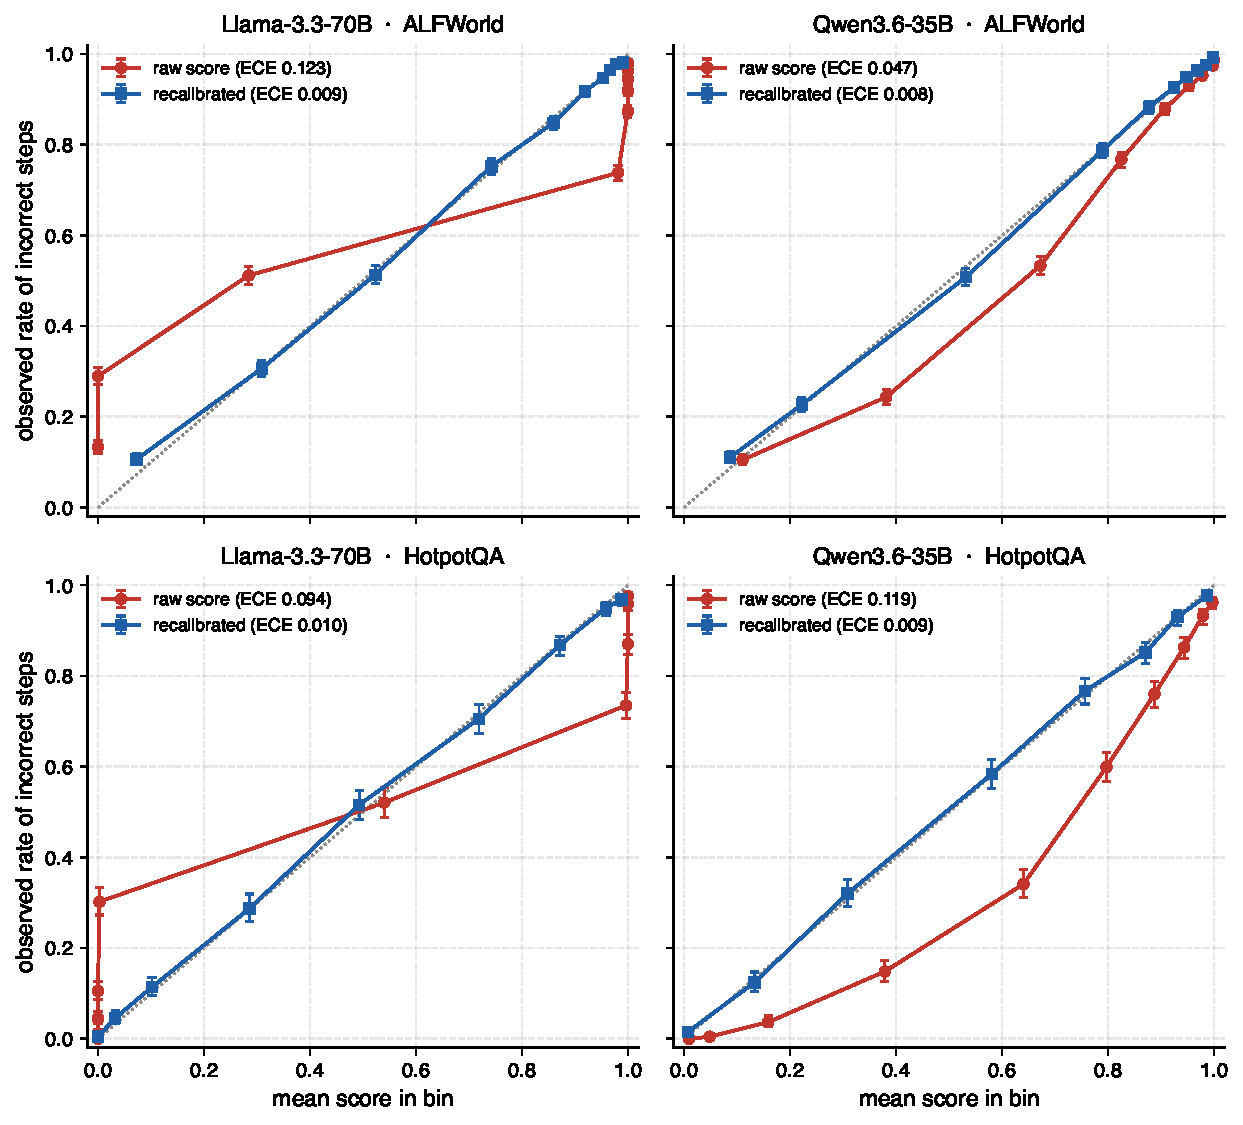
\includegraphics[width=0.95\linewidth]{fig_11_reliability.pdf}
\caption{Reliability diagrams per (estimator, environment), raw and after
isotonic recalibration fitted on the operating point's labelled episodes.}
\label{fig:reliability}\end{figure}
\begin{table}[t]
\centering
\small
\caption{Probabilistic calibration of the per-step scores, primary construct. ECE is over ten equal-mass bins; Brier and ECE under \emph{recalibrated} come from an isotonic map fitted on one half of the episodes and applied to the other, using the same episode split as the label-calibrated cut, so no additional annotation is spent. $\bar{y}$ is the cell's rate of incorrect steps; the constant column is the Brier score of predicting $\bar{y}$ for every step and the verdict column that of the estimator's own yes/no answer.}
\label{tab:calib}
\begin{tabular}{llrrrrrrrr}
\toprule
& & & & \multicolumn{2}{c}{ECE} & \multicolumn{2}{c}{Brier} & \multicolumn{2}{c}{Brier baselines} \\
\cmidrule(lr){5-6}\cmidrule(lr){7-8}\cmidrule(lr){9-10}
Estimator & Trajectory source & $n$ & $\bar{y}$ & raw & recal. & raw & recal. & constant & verdict \\
\midrule
\multicolumn{10}{l}{\emph{ALFWorld}} \\
Llama-3.3-70B & Llama-3.3-70B $^{\dagger}$ & 4285 & 0.53 & 0.193 & 0.022 & 0.210 & 0.155 & 0.249 & 0.228 \\
Llama-3.3-70B & Mistral-7B & 6203 & 0.80 & 0.121 & 0.012 & 0.130 & 0.103 & 0.160 & 0.143 \\
Llama-3.3-70B & Phi-4-mini & 6005 & 0.82 & 0.114 & 0.010 & 0.118 & 0.097 & 0.145 & 0.125 \\
Llama-3.3-70B & Qwen3.6-35B & 2872 & 0.42 & 0.287 & 0.055 & 0.299 & 0.201 & 0.244 & 0.314 \\
Llama-3.3-70B & DeepSeek-V4-Flash & 3067 & 0.34 & 0.174 & 0.031 & 0.201 & 0.154 & 0.224 & 0.219 \\
Llama-3.3-70B & Gemma-3-4B & 6507 & 0.91 & 0.038 & 0.008 & 0.059 & 0.051 & 0.082 & 0.063 \\
Qwen3.6-35B & Llama-3.3-70B & 4285 & 0.53 & 0.135 & 0.028 & 0.155 & 0.127 & 0.249 & 0.230 \\
Qwen3.6-35B & Mistral-7B & 6203 & 0.80 & 0.021 & 0.012 & 0.100 & 0.099 & 0.160 & 0.136 \\
Qwen3.6-35B & Phi-4-mini & 6005 & 0.82 & 0.057 & 0.008 & 0.097 & 0.092 & 0.145 & 0.128 \\
Qwen3.6-35B & Qwen3.6-35B $^{\dagger}$ & 2872 & 0.42 & 0.149 & 0.035 & 0.243 & 0.224 & 0.244 & 0.366 \\
Qwen3.6-35B & DeepSeek-V4-Flash & 3067 & 0.34 & 0.104 & 0.039 & 0.149 & 0.142 & 0.224 & 0.212 \\
Qwen3.6-35B & Gemma-3-4B & 6507 & 0.91 & 0.011 & 0.005 & 0.051 & 0.052 & 0.082 & 0.064 \\
\midrule
\multicolumn{10}{l}{\emph{HotpotQA}} \\
Llama-3.3-70B & Llama-3.3-70B $^{\dagger}$ & 1878 & 0.18 & 0.090 & 0.019 & 0.120 & 0.095 & 0.149 & 0.130 \\
Llama-3.3-70B & Mistral-7B & 2626 & 0.56 & 0.143 & 0.017 & 0.151 & 0.117 & 0.246 & 0.166 \\
Llama-3.3-70B & Phi-4-mini & 2282 & 0.57 & 0.097 & 0.012 & 0.125 & 0.099 & 0.245 & 0.139 \\
Llama-3.3-70B & Qwen3.6-35B & 1787 & 0.11 & 0.069 & 0.018 & 0.088 & 0.069 & 0.095 & 0.095 \\
Llama-3.3-70B & Gemma-3-4B & 2248 & 0.48 & 0.114 & 0.029 & 0.124 & 0.100 & 0.250 & 0.136 \\
Qwen3.6-35B & Llama-3.3-70B & 1878 & 0.18 & 0.169 & 0.007 & 0.143 & 0.098 & 0.149 & 0.216 \\
Qwen3.6-35B & Mistral-7B & 2626 & 0.56 & 0.135 & 0.017 & 0.146 & 0.120 & 0.246 & 0.206 \\
Qwen3.6-35B & Phi-4-mini & 2282 & 0.57 & 0.084 & 0.014 & 0.104 & 0.090 & 0.245 & 0.148 \\
Qwen3.6-35B & Qwen3.6-35B $^{\dagger}$ & 1787 & 0.11 & 0.110 & 0.015 & 0.086 & 0.066 & 0.095 & 0.121 \\
Qwen3.6-35B & Gemma-3-4B & 2248 & 0.48 & 0.096 & 0.013 & 0.106 & 0.090 & 0.250 & 0.153 \\
\midrule
\emph{pooled} Llama-3.3-70B & ALFWorld (5 cells) & 24654 & 0.73 & 0.123 & 0.009 & 0.137 & 0.106 & --- & --- \\
\emph{pooled} Qwen3.6-35B & ALFWorld (5 cells) & 26067 & 0.73 & 0.047 & 0.008 & 0.102 & 0.095 & --- & --- \\
\emph{pooled} Llama-3.3-70B & HotpotQA (4 cells) & 8943 & 0.45 & 0.094 & 0.010 & 0.125 & 0.098 & --- & --- \\
\emph{pooled} Qwen3.6-35B & HotpotQA (4 cells) & 9034 & 0.46 & 0.119 & 0.009 & 0.125 & 0.100 & --- & --- \\
\bottomrule
\end{tabular}
\\[2pt]\footnotesize $^{\dagger}$ the estimator reading its own trajectories; pooled rows exclude those cells.
\end{table}


\section{Matched-capability independence analysis}\label{app:matched}
Removing the family confound leaves the external advantage intact (same-family
reading of the held-out agents: $+0.059$ mean AUROC, 4/4 cells, all intervals
excluding zero). Removing the capability advantage removes most of it
(peer-scale mean $+0.008$, external ahead in 1 of 4; sub-7B estimators reading
one another: $-0.074$, ahead in 4 of 12, with 11 of 12 intervals excluding
zero, most favouring self-assessment). The peer-scale asymmetry (one direction
$+0.068$, the reverse $-0.007$ on the same environment) is the signature of
self-leniency rather than reader quality. Reader capability dominates what external reading buys, with evidence of
a smaller average self-leniency effect.
\begin{table}[t]
\centering
\small
\caption{What an external reading buys once the two confounds in the headline comparison are removed. $\Delta$ is the external reader's AUROC minus the agent's own best self-assessment, on identical steps, with a 95\% episode-clustered bootstrap interval. The self baseline is the best of the agent's four reading scopes, chosen in hindsight, which can only favour it. Primary construct.}
\label{tab:matched}
\begin{tabular}{lllrrrr}
\toprule
Environment & External reader & Agent read & $n$ & external & self (best) & $\Delta$ [95\% CI] \\
\midrule
\multicolumn{7}{l}{\emph{Same family: the family confound removed}} \\
ALFWorld & Qwen3.6-35B & Qwen3.5-4B & 3754 & 0.767 & 0.665 & $+0.102$ [$+0.079$, $+0.127$] \\
HotpotQA & Qwen3.6-35B & Qwen3.5-4B & 1914 & 0.922 & 0.877 & $+0.045$ [$+0.031$, $+0.059$] \\
ALFWorld & Qwen3.6-35B & Qwen3.5-9B & 3859 & 0.781 & 0.728 & $+0.053$ [$+0.036$, $+0.071$] \\
HotpotQA & Qwen3.6-35B & Qwen3.5-9B & 1202 & 0.911 & 0.876 & $+0.035$ [$+0.018$, $+0.053$] \\
ALFWorld & Qwen3.6-35B & Qwen3.5-27B & \multicolumn{4}{l}{\emph{no usable paired cell (single class or <40 shared labelled steps)}} \\
HotpotQA & Qwen3.6-35B & Qwen3.5-27B & \multicolumn{4}{l}{\emph{no labelled steps for this agent}} \\
\midrule
\multicolumn{7}{l}{\emph{Matched scale: the larger-judge confound removed}} \\
ALFWorld & Qwen3.6-35B & Llama-3.3-70B & 4285 & 0.897 & 0.904 & $-0.007$ [$-0.024$, $+0.010$] \\
ALFWorld & Llama-3.3-70B & Qwen3.6-35B & 2872 & 0.762 & 0.694 & $+0.068$ [$+0.036$, $+0.098$] \\
HotpotQA & Qwen3.6-35B & Llama-3.3-70B & 1878 & 0.893 & 0.902 & $-0.009$ [$-0.026$, $+0.008$] \\
HotpotQA & Llama-3.3-70B & Qwen3.6-35B & 1787 & 0.903 & 0.921 & $-0.018$ [$-0.035$, $-0.002$] \\
\midrule
\multicolumn{7}{l}{\emph{Small reading small: externality without capability}} \\
ALFWorld & Mistral-7B & Phi-4-mini & 6005 & 0.620 & 0.547 & $+0.073$ [$+0.046$, $+0.099$] \\
ALFWorld & Mistral-7B & Gemma-3-4B & 6507 & 0.730 & 0.668 & $+0.062$ [$+0.029$, $+0.094$] \\
ALFWorld & Phi-4-mini & Mistral-7B & 6203 & 0.468 & 0.646 & $-0.179$ [$-0.209$, $-0.148$] \\
ALFWorld & Phi-4-mini & Gemma-3-4B & 6507 & 0.514 & 0.668 & $-0.155$ [$-0.195$, $-0.114$] \\
ALFWorld & Gemma-3-4B & Mistral-7B & 6203 & 0.421 & 0.646 & $-0.226$ [$-0.257$, $-0.194$] \\
ALFWorld & Gemma-3-4B & Phi-4-mini & 6005 & 0.412 & 0.547 & $-0.136$ [$-0.163$, $-0.108$] \\
HotpotQA & Mistral-7B & Phi-4-mini & 2282 & 0.704 & 0.632 & $+0.072$ [$+0.045$, $+0.097$] \\
HotpotQA & Mistral-7B & Gemma-3-4B & 2248 & 0.727 & 0.751 & $-0.024$ [$-0.049$, $+0.001$] \\
HotpotQA & Phi-4-mini & Mistral-7B & 2626 & 0.540 & 0.769 & $-0.229$ [$-0.253$, $-0.205$] \\
HotpotQA & Phi-4-mini & Gemma-3-4B & 2248 & 0.595 & 0.751 & $-0.156$ [$-0.183$, $-0.129$] \\
HotpotQA & Gemma-3-4B & Mistral-7B & 2626 & 0.677 & 0.769 & $-0.093$ [$-0.116$, $-0.069$] \\
HotpotQA & Gemma-3-4B & Phi-4-mini & 2282 & 0.729 & 0.632 & $+0.097$ [$+0.072$, $+0.122$] \\
\midrule
\multicolumn{7}{l}{\emph{Boundary: the cells where self-assessment is not beaten}} \\
HotpotQA & Qwen3.6-35B & Llama-3.3-70B & 1878 & 0.893 & 0.902 & $-0.009$ [$-0.026$, $+0.008$] \\
HotpotQA & Llama-3.3-70B & Qwen3.6-35B & 1787 & 0.903 & 0.921 & $-0.018$ [$-0.035$, $-0.002$] \\
\bottomrule
\end{tabular}
\end{table}


\subsection*{Figures}
\begin{figure}[t]\centering
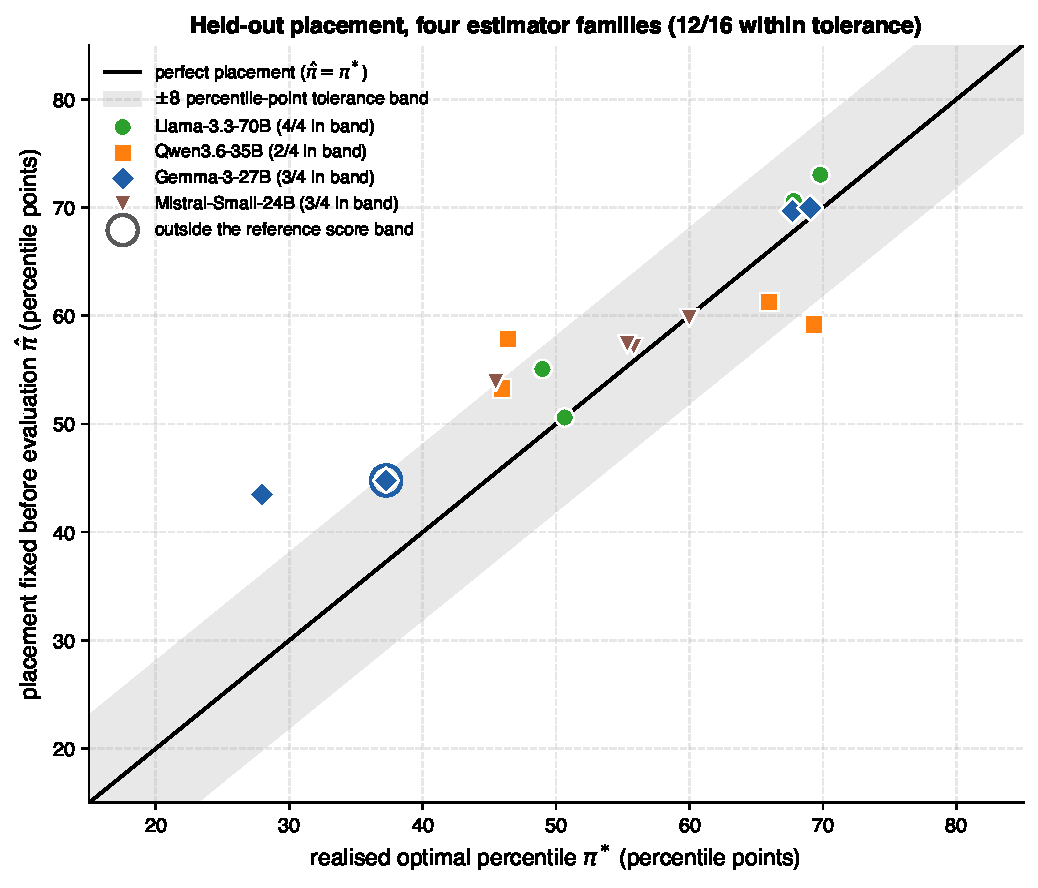
\includegraphics[width=0.98\linewidth]{fig_8_forecast_scatter.pdf}
\caption{Held-out placement across four estimator families. Each point is one
evaluable held-out agent: horizontal, the optimal cut percentile the labels
turned out to require; vertical, the percentile fixed before any of those
labels were read. The shaded band is the $\pm 8$-point tolerance; 12 of 16
cells fall inside it, zero labels spent on the target. Rings mark cells whose
mean score lies outside the reference band, where the interpolation-only
scope condition does not license deployment; the two later estimators were
the weakest qualifiers, and their misses fall where reference scores
compress.}\label{fig:forecast}
\end{figure}
\begin{figure}[t]\centering
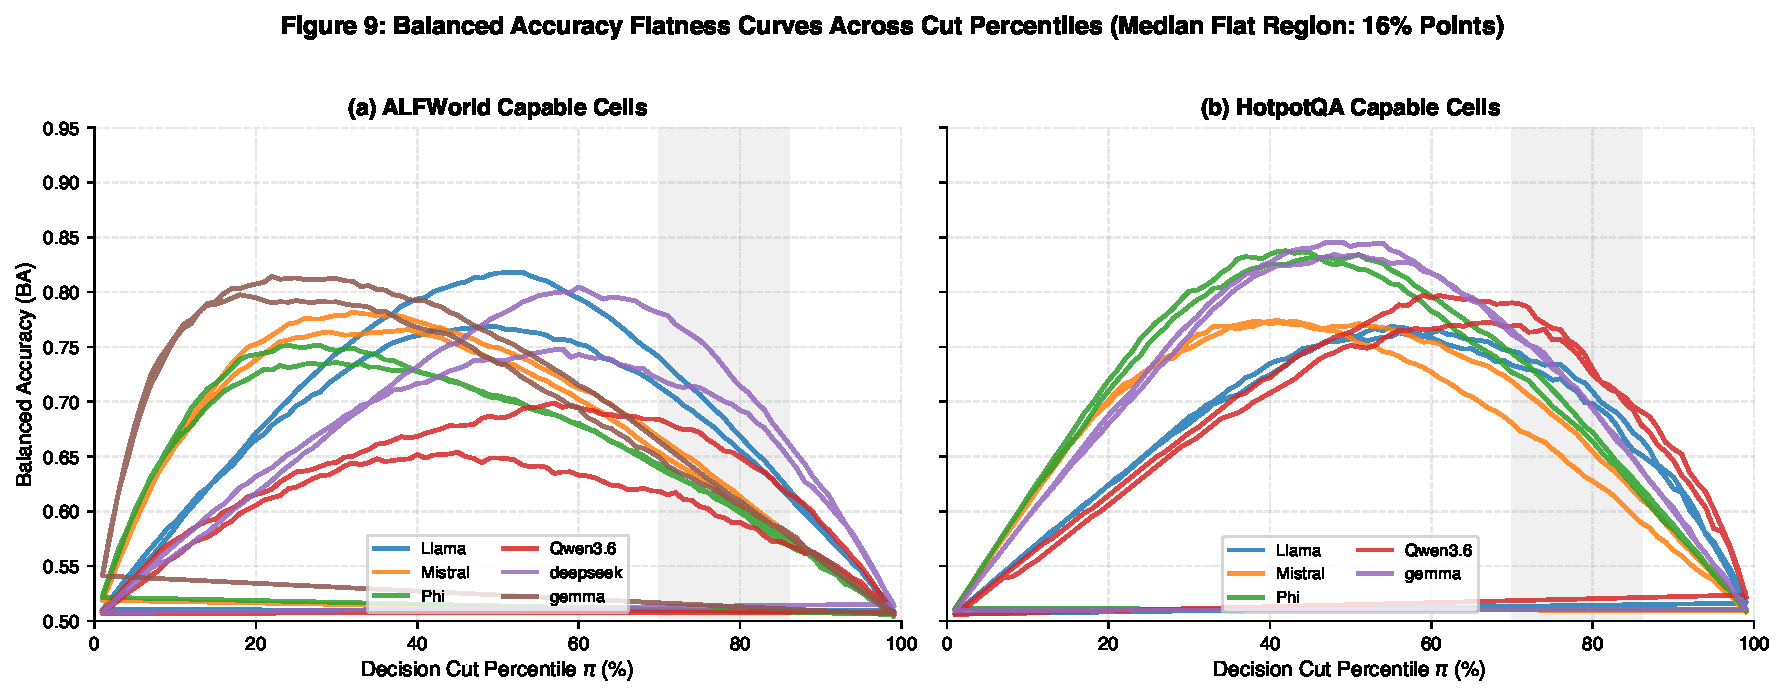
\includegraphics[width=0.98\linewidth]{fig_9_flatness_curves.pdf}
\caption{Balanced accuracy versus cut percentile per capable cell: the median flat region spans 16 percentile points, the error budget the operating-point map must meet.}\label{fig:flatness}
\end{figure}
\begin{figure}[t]\centering
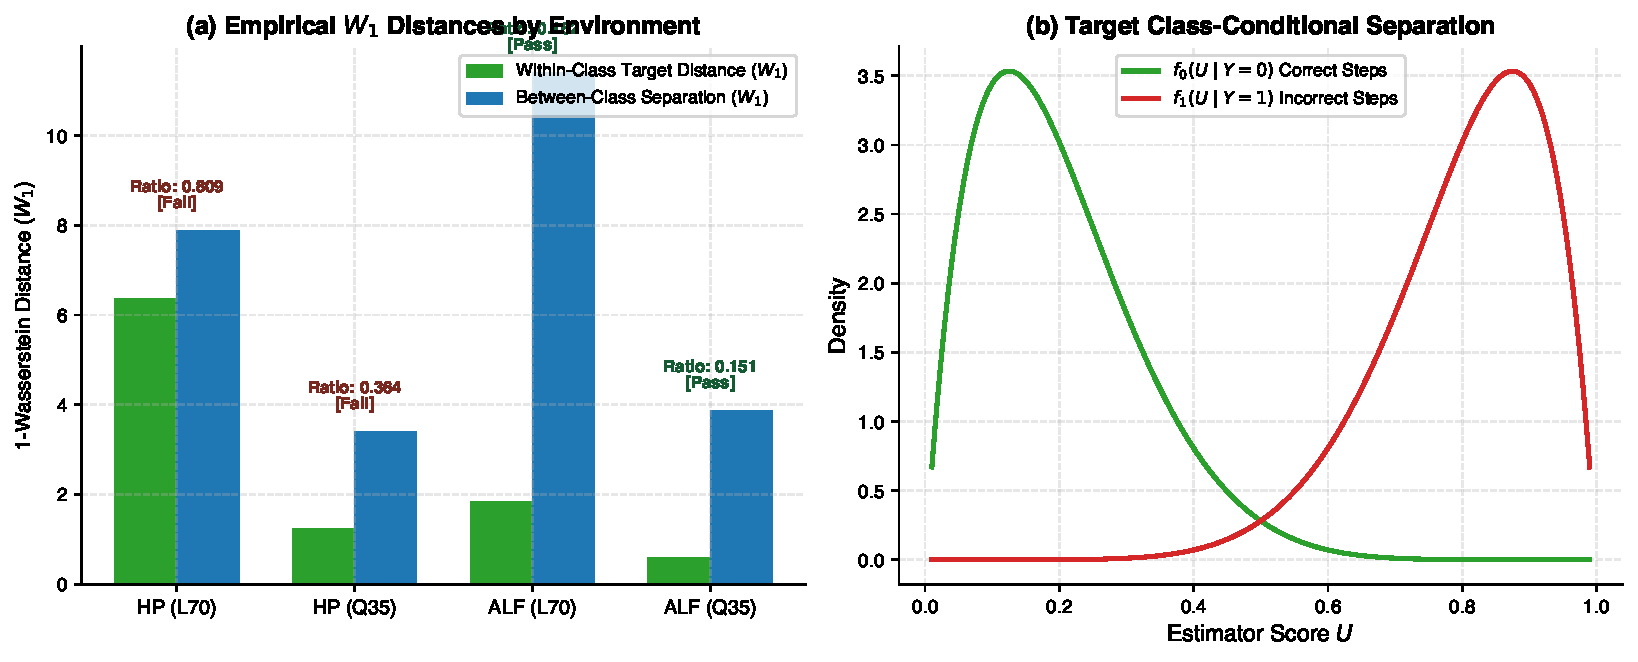
\includegraphics[width=0.98\linewidth]{fig_10_conditional_invariance.pdf}
\caption{Class-conditional score distributions across targets: approximate invariance on HotpotQA, failure on ALFWorld, where the map nevertheless works; the mechanism is the flat landscape plus a coarse affine regularity.}\label{fig:invariance}
\end{figure}
\begin{figure}[t]\centering
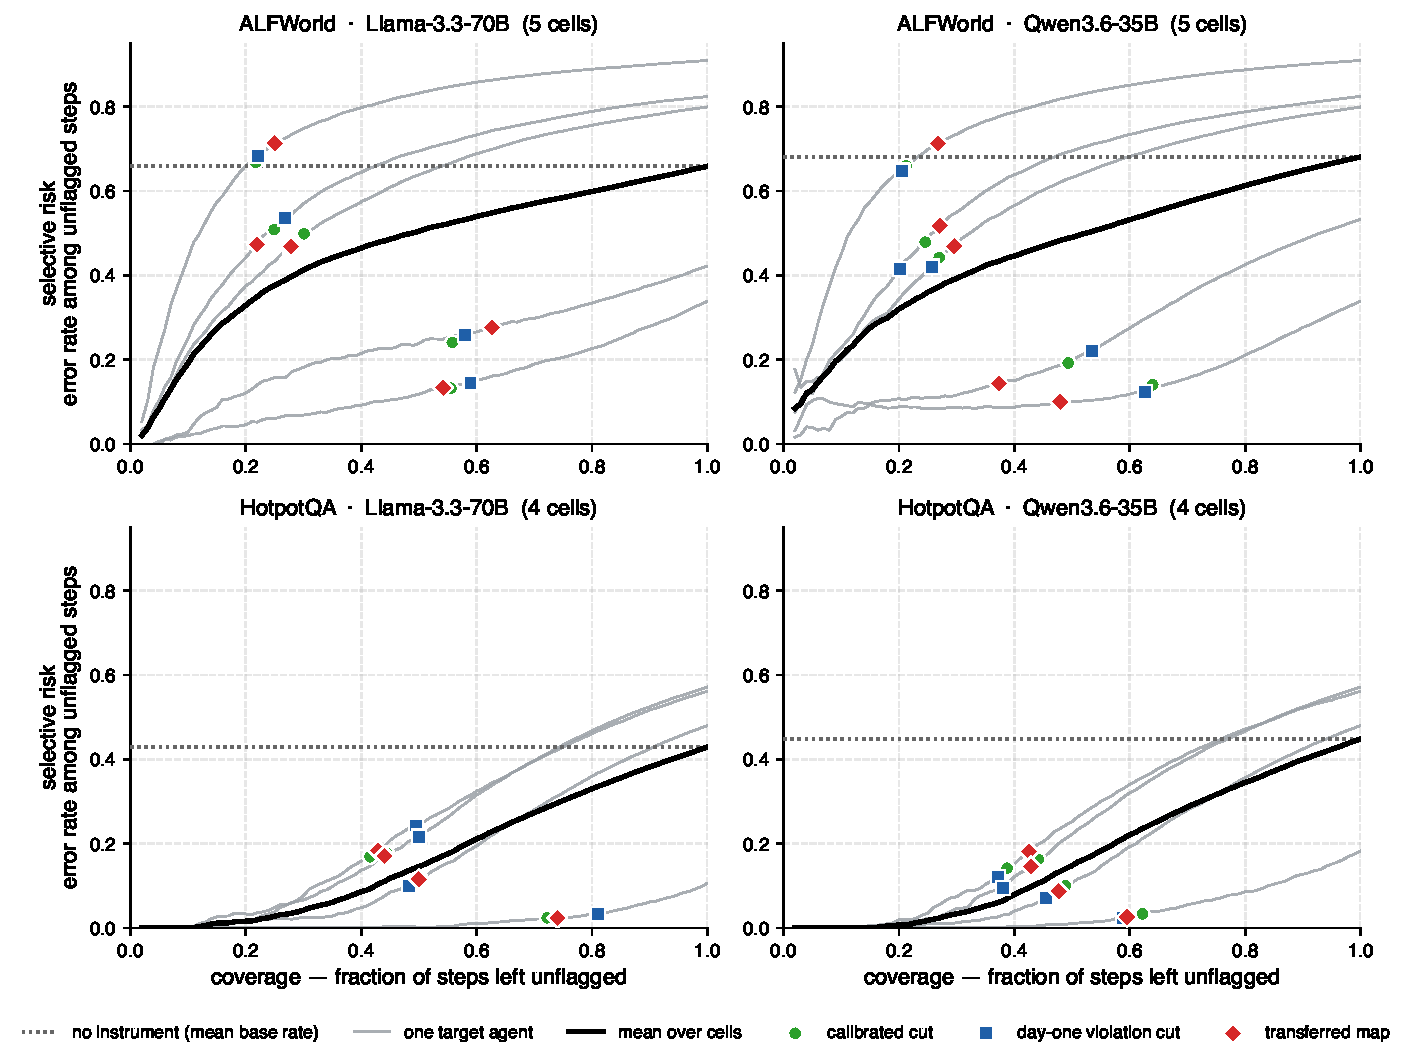
\includegraphics[width=0.92\linewidth]{fig_13_risk_coverage.pdf}
\caption{Selective risk versus coverage per (estimator, environment), with
the three deployment routes' operating points marked; they coincide on the
curve.}\label{fig:riskcoverage}\end{figure}
\end{document}
